\chapter{Solution}


\section{Oveview} 


\subsection{Work Produced}

The \textbf{Figure \ref{fig:schema}} show the overview and the main flow of the overall application.
The Overall System and the work produced to create the application is composed by the following parts:
\begin{outline}
    \1 \textbf{Networks}: It's the networks over that the blockchains runs. The project involves two kind of networks:
    \2 \textbf{Hyperledger Fabric Network}: It's the main network used for own project.
    \2 \textbf{Ethereum Network}: It's the side network used for token exchanged for own use. In that 
    project is used the testnet Ropsten.    
    \1 \textbf{Shell Scripts}: to allow to setting up everything in the best way, It's produced a set of 
    shell scripts that run network or shut down it, install chaincode, and run part of the system mandatory 
    for the application use. 
    \1 \textbf{Smart Contracts}: The smart contracts perform project use cases actions. 
    There's three smart contracts and each of that perform one specific flow and involves just
    a set of overall actors of the system.  
    \1 \textbf{Dapp}: It's the web application used to allow actors to interact with the system. It's a
    decentralized application that communicate with the blockchain networks. Once the user is logged in with 
    related privileges, could perform smart contracts invokation using the web-app.
\end{outline}

\subsection{Actors}

The main \textbf{Actors} involved in the system are three:

\begin{outline}
    \1 \textbf{User}: It's the \textit{end user}. It use the web-app to send old clothes and purchase from Reclothes store.
    The User is the Actor that start the entire process flow, \textit{sending the clothes}, mandatory for the entire process. 
    \1 \textbf{Reclothes Admin}: It's the \textit{system admin}, it perform the actions in order to handle the system.
    The Reclothes Admin handle both parts User Side and Producer Side. About User Side It perform a set of actions
    in order to handle in the best way the clothes arrived and the tokens provided. On the other hand, Producer Side,
    it cares about to handle the recycling and upcycling process, providing to the Producer old materials
    and spend, when the platform needs, the token received to order recycled clothes.  
    \1 \textbf{Producer}: It's part of the upcycling process. It receive the materials to perform the recycling process.
    In our use case test we consider just one Producer that receive the entire old materials to be recycled.
    However the system is developed in order to allow a set of Producers registered and the Reclothes Admin
    during the \textit{Send Old Clothes} process could choose the Producer that prefer. 
\end{outline}

\subsection{Application Flow}

Each Actors access to the system wich different permission and priviledges. Once the user is logged in, 
It could access to several features and is allowded to perform a set of actions over the system. 
For a better understanding we are going to split the overview flow shown in \textbf{Figure \ref{fig:schema}} 
into 2 subflow starting from Reclothes actor, considered as the \textit{System Admin}, 
the \textbf{User side} on the left side and the \textbf{Producer side} on the right side. 

\bigskip

Each side has a set of main actions that going to modify the world state of the blockchains.
Based on that principle the smart contract invocations that going to produce transactions modifing the 
ledgers in an immutable way, adding a new block to the chains, are the following one: 

\begin{outline}[enumerate]
	\1 \textbf{User Side}
    \2 User send Box with old clothes and receive Fabric points and ERC20 Token
    \2 User purchase items inside dapp store using Fabric points and ERC20 Token
    \1 \textbf{Producer Side}
    \2 Reclothes send clothes box with old matherials and receive Regeneration Credits
    \2 Reclothes spend the Regeneration Credits to purchase upcycled clothes by Producer
\end{outline}

That process going to be described in details in the \ref{use-cases} section that analyze 
deeper the transactions process. 

\subsection{Token echanged}

There are two \textbf{Token} categories exchanged over the networks. 
\bigskip

Over Hyperledger Fabric side going to be exchanged two kind of tokens, both are points based integrated with the 
smart contracts that handle User and Producer side both. The user points are going to be handle 
totally Reclothes side, it means that it's the Reclothes Admin to decide the amount to be send to the User. 
To handle the transactions amount and estabilish a standard behaviour it's need  
a reference table that set a fixed amount for each clothes received. The producer side 
points, \textit{Regeneration Credits}, are totally handled by Producer side, there's the producer that receive 
old materials and than choose the amount to be send. As the user points it needs a table to fix rules for 
the corrisponding amounts for received materials evaluation. 
\bigskip

On the other side, there's the ERC20 token that run over the ethereum network. ERC20 is a standard protocol
that allow to implement own token following fixed rules. That standard token includes a set of fixed
operations allowed over that, \texttt{totalSupply, balanceOf, transfer, transferFrom, 
approve and allowance}. 

\bigskip
For a better understanding of the exhanged token over own project, It's listed below:

\begin{outline}[enumerate]
	\1 \textbf{Over Fabric Network}
    \2 \textbf{User Token}: It's a token, points based, used to handle part of payment system related to clothes
    shipping from User to Reclothes and viceversa.
    \2 \textbf{Regeneration Credits}: It's a token, points based, used to handle part of credit system related to clothes
    shipping from Reclothes to Producers and viceversa.

    \1 \textbf{Over Ethereum Network}
    \2 \textbf{CO2 Token}: It's and ERC20 Token run over public network in charge to handle part of payments
    related to clothes shipping from User to Reclothes and viceversa.
\end{outline}


\begin{figure}[h!]
	\centering
	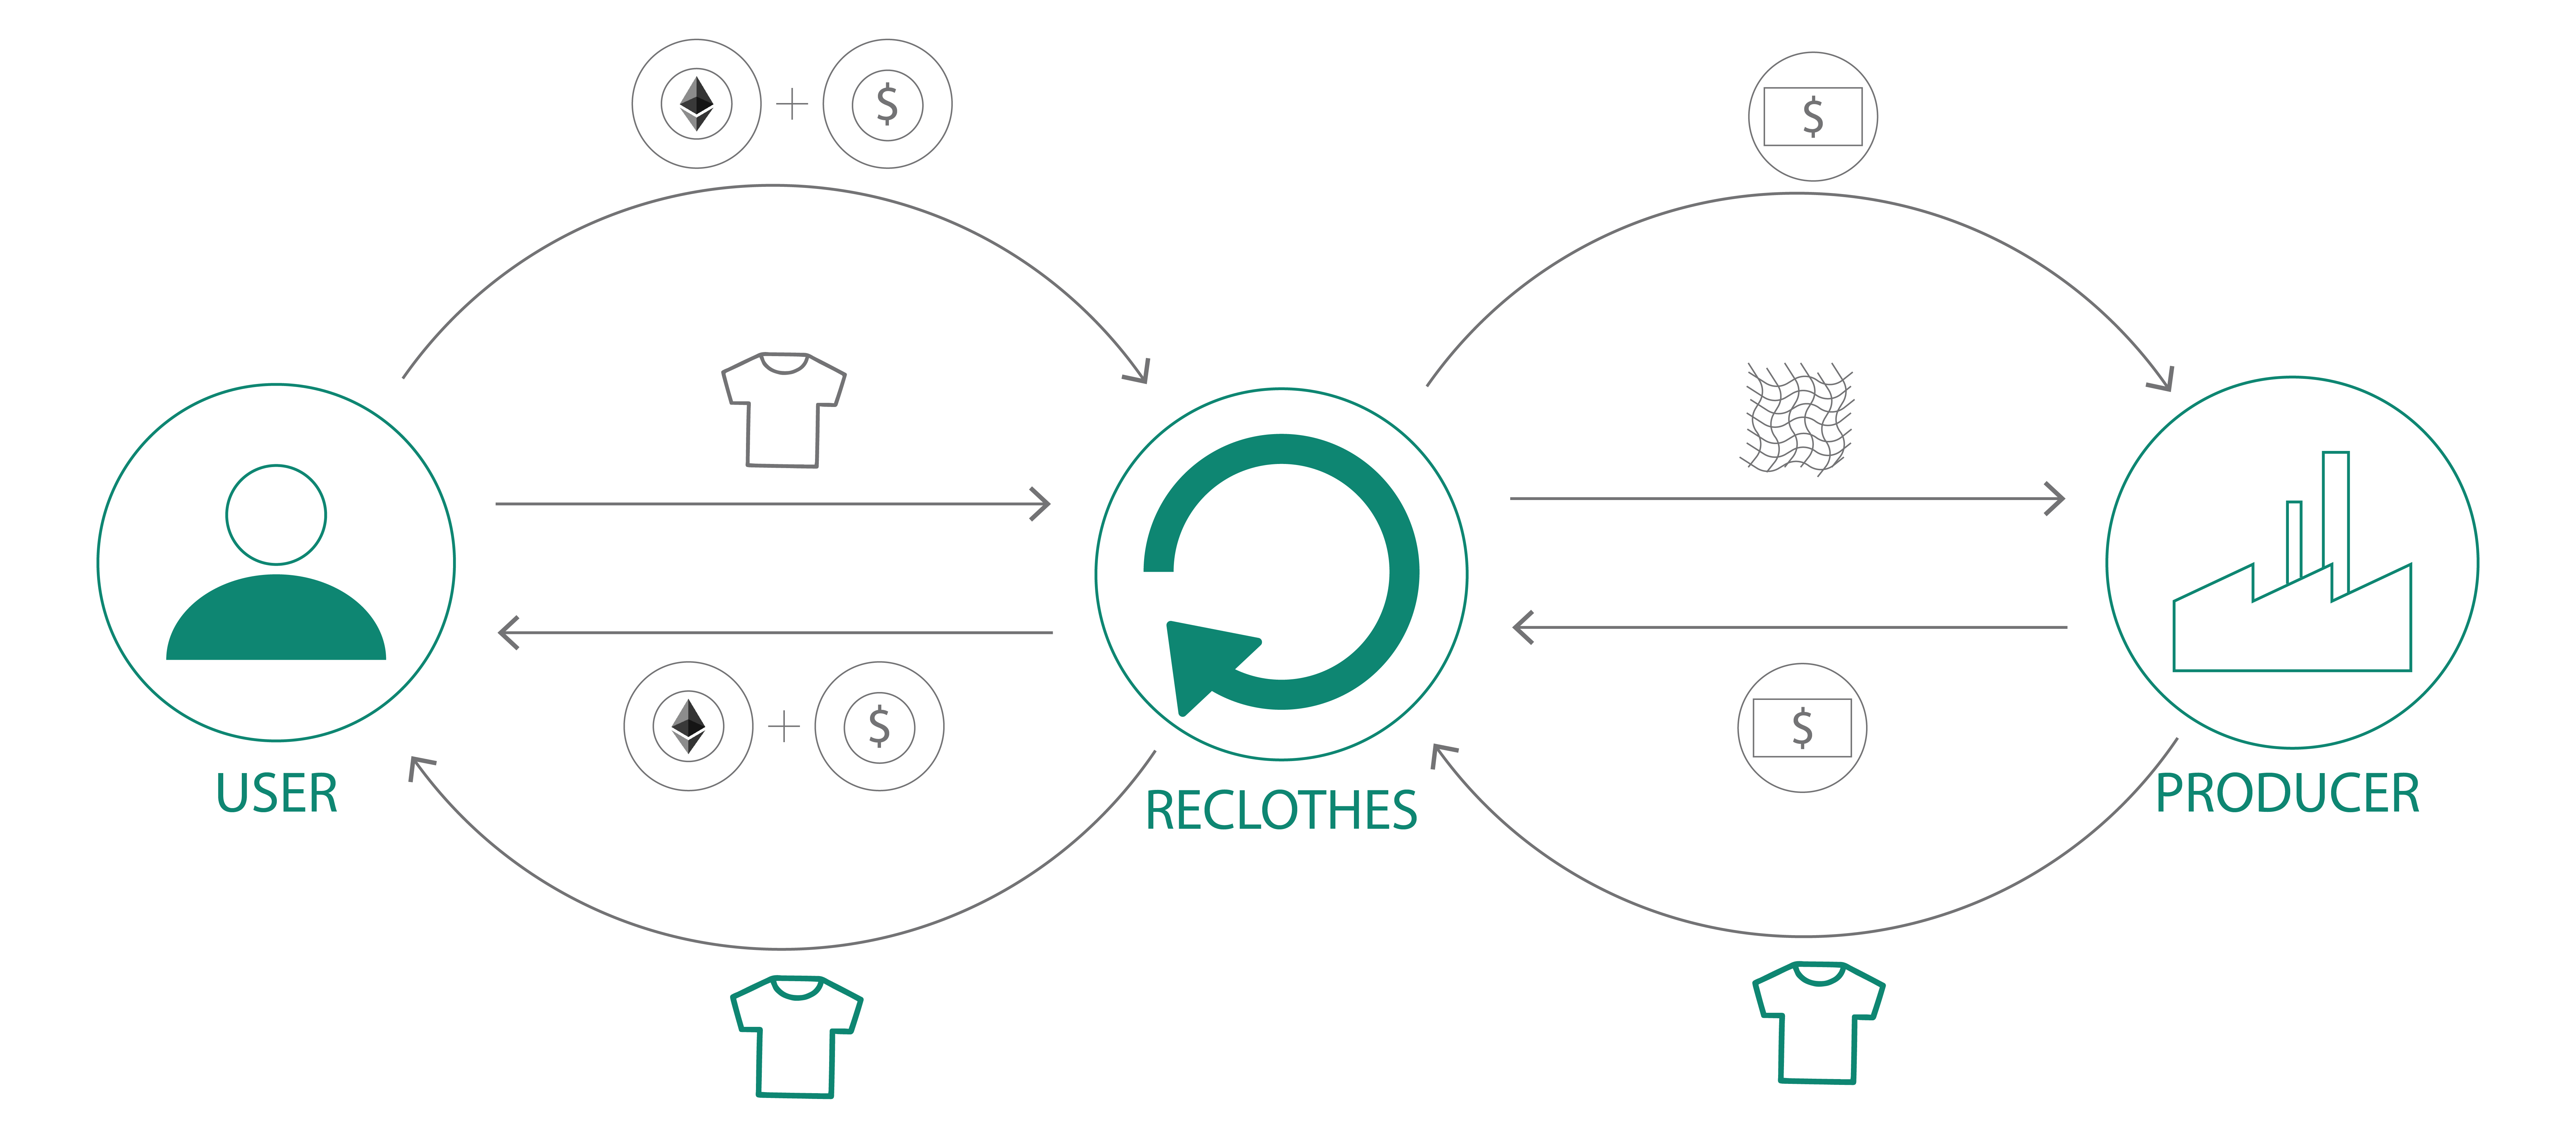
\includegraphics[totalheight=6cm]{img/use-case-schema.png}
	\caption{UseCase Overview}
	\label{fig:schema}
\end{figure}

%CROSSCHAIN
\clearpage
\section{Crosschain interaction}

\subsection{Why needs crosschain solution}

One of the goal of the project is to build a good integration between the two blockchains networks
involved in the system. The needs of a cross-chain solution applied to own use cases is to 
keep the \textbf{\texttt{CO\textsubscript{2} Token}} exchanged public, in order that for future use could be reused in 
other environment and applications. In that way the token is not strictly correlated to own personal use, but
It could became a standard token to be exchanged over ethereum, and corresponding to an asset
related to CO\textsubscript{2} emissions. The behaviour of that token going to be analized better
in \ref{erc20} section.
\bigskip

The requirements to obtain a good integration is to perform cross-chain
process without compromise the security issue both side, fabric and ethereum. Therefore we 
need to care about the technologies behaviour both and what's the technical basis upon which 
blockchains works. 
\bigskip

To understand the solution choosed, to perform the cross-chain interaction, it's need to understand the 
technologies that we used to develop the project.

\subsection{Technologies Used}

Below there's all the main technologies used, involved in application and crosschain process.
The \textbf{Figure \ref{fig:architectural-flow}} shows how that technologies and tools is used and
interact each other. 

\begin{outline}
    \1 \textbf{Metamask}: It's used as ethereum wallet to perform and sign the transactions started by dapp.
    It grant an high level of security to perform and sign transactions over the ethereum networks. It is 
    integrated in own project, application side, and for the right usage of the entire application, It's
    mandatory that the user is logged in Metamask over the wallet specified during registration phase.  
    \1 \textbf{Web3}: It's the software library used to interact with smart contract.
    Web3.js it's the API that enables the developers to fulfill the integration between website/client and ethereum blockchain.
    It is a collection of libraries that allow developers to perform actions like send Ether from one account to another, read 
    and write data from smart contracts, create smart contracts, and much more. 
    \1 \textbf{Fab3 Proxy}: It map the Web3 API with the Fabric SDK in order to interact with
    Fabric network. It perform a mapping between the Fabric Identity (X.509) with an eth address, generated on the fly,
    used to perform dapp call. In other world it works like a bridge between ethereum technologies and tools, used 
    for dapp development, and fabric chaincode, that run over the fabric peer and use the GO SDK to allow 
    the chaincode invocation.  
    \1 \textbf{Fabric Chaincode EVM}: It's the ethereum virtual machine chaincode that allow to run Solidity smart contract
    over the Fabric network. It's a core part of the entire project. Thanks to that chaincode is
    allowed to run solidity bytecode over fabric peers.
    \1 \textbf{Remix}: is an online editor that allow to develop well structured solidity smart contracts.
    Thanks to the plugins, that could be installed over the editor, it's possible to compile the wrote
    smart contracts code. Once the compiling process succed, it produce the corresponding smart contract's bytecode
    and the smart contract's ABI. Bytecode and ABI both are used to define the smart contract behaviours. 
    That parameters are passed as argument during the deployment process. 
    \1 \textbf{Expressjs}: Web Framework used to develop web-app and smart contract API.
    It's a light, easy and fast framework that integrates several methods usefull for HTTP and middleware API development. 
    \1 \textbf{Infura}: allow to run a Ethereum node in order to set an endpoint used to interact with own contract.
    It allow in an easy way to set up a public endpoint for own deployed contract address. It deliver personal 
    API and key for the endpoint access. Moreover it provide a really well defined and detailed dashboard
    to analyze all the smart contract invocations, providing deeper analisys for the called method too.  
    \1 \textbf{Docker}: The fabric network components run inside Docker containers. It's mandatory
    for fabric network blockchains, each peer(node) of the network run inside a specific and 
    dedicated container. It allow to be monitored and analized in an indipendent way. 
\end{outline}

Thanks to the introduction of the EVM chaincode developed by the IBM technical ambassador,
it's possible to run Solidity bytecode over the Fabric network. It allow the possibility to adopt 
ethereum technologies over Hyperledger Fabric Network.
That innovation doesn't improve only by the integration network side but client side too, because with the 
\texttt{fabric-chaincode-evm} it's opened a new communication way from dapp/client side to the network side.
The Web3 libraries is allowed to handle the smart contract invocation and all the most 
of the improvements done in the Ethereum environment, could be used to interact with 
Hyperledger Fabric world. It means languages, API, libraries and tools that by now founds a
huge application in ethereum reality.  
\bigskip

The CrossChain solution that I choose to implement, in the following Use Cases, involves the 
Application Layer.
The main core idea of the solution is to mapping, at application level, the ethereum Wallet with Hyperledger
Fabric Identity and use one for transactions over ethereum network and the other one over fabric network.
Exploiting Web3.js API we invoke ethereum or fabric smart contracts, using that solution all the invocation
processes going to be forward, to the corresponding network, starting Dapp Side. 
\bigskip

The security is granted Fabric Side using certificate x.509, the authentication mechanism doen't
change. Once the user is authenticated and recognized by own x.509 certificate, fabric network logged the user in 
to the platform and give him the access to the data informations and all the related privedges based 
on the actor Role.
\bigskip

On the other hand ethereum side is handled in the following way, the own ethereum public address is specified
during registration phase and saved over fabric chaincode to the corrisponding User data structure.
When the user is involved inside transaction processes, all the transactions reffer to the public ethereum
address reported during registration phase. 
\newline 

Therefore when there's an incoming transaction the tokens will be send to the public address reported in User Data infos. 
\newline

When there's an outgoing transaction, the security is granted thanks to the Metamask integration during the transaction process. At the 
moment of transactions the sign, that allow to perform transaction, is performed Metamask side, in that way only the real owner of the ethereum account
could sign and approve the transaction. The private key is stored over metamask wallet and just the real
owner that is logged in to the own account could perform the sign of the transaction. 
\bigskip

\textbf{Figure \ref{fig:architectural-flow}} shows The Architectural Flow and how the technologies is used and interact each other.

Metamask is used as ethereum wallet to sign transaction over ethereum network, In the entire project we suppose
that the Actor is logged in over Metamask account reported during registration phase. It is collocated
at browser layer of the architectural flow.  

Furthermore, fabric side the actor is logged over fabric network using standard fabric authentication
process, spending own x.509 certificate. Therefore the Dapp client show the access to the actor page.
The dapp client use Fab3 Proxy to map the identity from eth address to fabric
identity x.509 certificate and forward request to fabric network, that process is indipindent by the ethereum address
specified during registration phase and doesn't interact with that. Fab3 allow to use \texttt{fabric-chaincode-evm} 
and run solidity code over fabric network, It perform a mapping process amoung the received requests dapp side.
Fab3 receive the Web3 request and map it using the GO SDK in order to forward in the right way all the request
to the Fabric peer. 
\bigskip

Moreover the Dapp client talk with ethereum public blockchain network, using the network endpoint api supplied by Infura. 
For some kind of actions performed over the platform, part of the request are going to be forward over
ethereum network. 

\begin{figure}[h]
	\centering
	\includegraphics[totalheight=14cm]{img/architectural_flow.png}
	\caption{Architectural Flow}
    \label{fig:architectural-flow}
\end{figure}
 

%USE CASES
\clearpage
\section{Use Cases}
\label{use-cases}

As specified in the previous sections, for a better outline we are going to split the use cases
inside the \textbf{User Side} and the \textbf{Producer Side}. The main actor of the system
remain Reclothes Admin that is linked to the both side and interacts with all the other
actors in order to supply the management support that allow the entire system works.

\subsection{UseCase 1 - User Side}

As shown in \textbf{Figure \ref{fig:usecase1}} both Actors User and Reclothes Admin, once is logged in, access to a set
of features. The Use case diagram show all the action that both users could perform over the networks and
the flows that each actions follow. The features are split over the two network, the Fabric one and the 
Ethereum one. All the flows start from one of the two actors involved and at the end merge to the one 
of the two blockchain networks. Each actor has a dedicated Ethereum wallet used for ethereum token
transaction. 
\bigskip

We are going to analyze all the actions that users coul perform over the system:
\begin{outline}
    \1 \textbf{Actions in common}
    \2 \textbf{Registration}: The registration phase involves the actor that fill a form with all the 
    mandatory data. To proceed to a successfull registration process it's mandatory that the actor
    owns the appropriate x.509 certificate, released by the certification authority related to the Role
    in which the user try to sign up. For example User has a specific Certification Authority that is
    different by the Reclothes CA. 
    \2 \textbf{Sign In}: The sign in is authomatic once the fabric network recognize the certificate and 
    logged in as the correspondic actor, once is logged in, the chaincode is invoked and going to read the 
    ethereum address used for the registration phase and provide the access to the methods.
    In other world fabric certificate provide the access to the network (peers, channels and ledger),
    instead the ethereum address used provide the access to the smart contract. 
    
    \1 \textbf{User Operations}
    \2 \textbf{Read Operations}
    \3 \textbf{View own transactions}: The User, once is logged in, could view all the own transactions
    processed by the network, with a flag that show transaction status. The trasactions includes token 
    exchanged over the network and box request sent to Reclothes. It give the possibility to 
    monitor and manage each process in which user is involved. 
    \2 \textbf{Write Operations}
    \3 \textbf{Send Box}: It's the starting point of the overall application flow. In the following subsection
    we going deeper in order to explain how that process works and what transactions depends by that.
    \3 \textbf{Purchase Items}: It's a write operations, belong of that start a transaction process. in that
    process is involved both the networks. Even that is explained deeper in the followinf subsection.

    \1 \textbf{Reclothes Admin Operations}
    \2 \textbf{Read Operations}
    \3 \textbf{View all transactions}: The Reclothes Admin, once is logged in, could view all the transactions
    processed by the network related to all the users involved, with a flag that show transaction status. The trasactions includes token 
    exchanged over the network. It give the possibility to monitor and manage each process in which there's a token transactions
    for analysis aim.
    \3 \textbf{View All Box Requests}: The Admin is allowed to analyze the process of the box shipping.
    The box data structure include all the relevant data, moreover it includes a flag that specify the status
    of the request, that flag could be \texttt{Pending, Evaluated}. 
    \2 \textbf{Write Operations}
    \3 \textbf{Evaluate Box}: Even this process belong to write operation, beacuse it start a transaction
    process that going to be write the blockchain world state. 

\end{outline}


The main action of the overall system is the send box operation performed by the user towards to Reclothes.
It's the starting point of the overall flow. The Internal Flow of the \textit{\bf{Send Box}} macro 
process, and what that process belongs, is the follow one:

\begin{outline}[enumerate]
    \1 User send box with old clothes
    \1 Reclothes Admin receive box, evaluate it
    \1 The web app perform the payments from Reclothes Account to User Account
    \1 Once both transactions succed, both token are accredited and User could spend it
\end{outline}

\subsubsection{Transactions}

In that first Use Case are involved both the blockchain networks. The main part and the most critical
one is the transaction action. Considering always \textit{Reclothes Admin} the
main actor of the system, there's two kind of transaction in which admin is involved. 
The \texttt{outgoing} transaction that starting by \texttt{Evaluation} process performed by the Reclothes Admin
once it receive the clothes box sent by the user. The other one is the \texttt{incoming} transaction,
in that case the token are exchanged from the User to the Reclothes Admin. The action that start
the incoming transaction process is the \texttt{Purchase Item} performed by the Users over the platform store.
\bigskip

The outgoing and incoming transactions are strictly correlated due to the token flow. As we told in the 
previous section the main and first one action is the \texttt{Send Box} that involve the \texttt{Evaluation}.
The Evaluation is the first outgoing transaction process over the system. Once the token are moved from the Reclothes Admin,
the User is allowed to use application and purchase items over it. 

\begin{outline}[enumerate]
    \1 The \textit{\bf{Evaluation}} process works in the following way:
    \2 Reclothes Admin visualize the next pending request to be evaluated. The Admin visualize all the related informations
    associated to the box request: \texttt{userAddress} it's the ethereum user address of the sender, 
    \texttt{tshirt, pants, jacket, other} with the related number of items associated to the request,
    and the status of the request, at this point still \texttt{In Pending}.
    \2 Reclothes Admin evaluate it. For a better evaluation process is proposed a solution based on
    a reference table with a fixed amount for each items, related to the clothes status. 
    At that points there's a filtering process, each items inside the box, is filtered based on 
    platform criteria. Than the Admin decide the status of the clothes and its final desination (platform store or recycling material).
    Once that the overall clothes was been evaluated and there's been set a total amount value 
    of Fabric points and ERC20 Token, the transaction process could start.
    \3 The Fabric points are sent over Fabric network invoking the chaincode function \texttt{sendPoints(address toAddress)}.
    That function accredited the specified amount of fabric points, updating the User balance. 
    \3 The ERC20 Token are send over Ethereum network, during the project development we are going to 
    use the Ropsten testnet to exchange the token. There's a previous step before performing
    token transaction, the fabric chaincode is invoked in order to obtain the ethereum address related to 
    the sender box user. Once that the fabric chaincode return the ethereum account, stored
    in the smart contract during the User Registration Phase, the application perform the transfer 
    of the ERC20 token from the Reclothes wallet to the User ethereum wallet
    \2 Once both transactions succed, both the transaction return to the application and it's performed
    an additional check in order to synchronize both transactions. Tokens are accredited and 
    informations about balances are going to be update. From that moment the User could spend the received
    tokens over the platform store, performing purchasing. 

    \1 The \textit{\bf{Purchase Items}} process works in a similar way but inverting the previous flow:
    \2 User choose the items to purchase over the web-app store. The items (tshirt, pants, jacket or other) 
    is represented with the related form reporting all the relevant informations. over the chaincode
    the smart contract store a dedicated data structure for storing clothes data informations. 
    The related price is expressed through tokens, fabric tokens and CO\textsubscript{2} tokens both. 
    \2 Once the items is choosed, start the purchase process. The User send the fabric tokens over fabric
    network and the CO\textsubscript{2} token over ethereum network. First of all there's been executed
    a set of controls in order to check both the balances and evaluate if the User could perform
    the purchase transaction. Once that all the check is passed correctly the both transaction starts
    each over own network. Once the transfer process is performed the smart contracts return the 
    operation results to the dapp, that communicate with a message the results of the operations.
    \2 If the transfers succed, both the tokens balance going to be update and the User could
    continue to perform actions over the platform.    
\end{outline}

\begin{figure}[h!]
	\centering
	\includegraphics[totalheight=15cm]{img/use_case1.png}
	\caption{UseCase 1}
	\label{fig:usecase1}
\end{figure}


\subsection{UseCase 2 - Producer Side}

The Use Case 2 is related to the right side of the overall flow schema shown in Figure \ref{fig:schema}.
It shape interactions between Reclothes Admin and Producers. For a better understanding of the process 
involved in that interaction, the Use case 2 diagram is shown in \textbf{Figure \ref{fig:usecase2}}.
In this case all the features are performed over the Hyperledger Fabric network, so there's no 
a crosschain part. The token exchanged, \texttt{Regeneration Credit}, is based over fabric smart contract
 and it's point based, without the needs to involve the ethereum blockchain.

\bigskip 
Going to analyze the Figure \ref{fig:usecase2}, even here there's the main action that leads to a transaction
process. Looking at the diagram we could split the flow into two subflow, the first one from Reclothes
 to Producer. In that subflow we cound identify two main actions \textbf{\texttt{\textit{Send Box}}} and \textbf{\texttt{\textit{Purchase Box}}}, 
 as specified in the previous use case, these are the operation that perform a world state update of the 
 blockchain ledger. on the other hand, in the second subflow, from Producer to Reclothes, is involved just 
 one action that produce al outgoing token transfer, the \textbf{\texttt{\textit{Evaluate Material}}} function. 

\bigskip 
All the asset exchange is handle using \textbf{Regeneration Credits} a Fabric token exchanged
and handle by the Fabric chaincode and running over Fabric network. To test our use case we consider
just one Producer that perform the overall recycling process, even if the smart contract is structured
in order to allow the handling and management of more Producer actors involved in the system. In case
of many Producers us involved in the recycling process, an ERC20 integration to handle the Regeneration
Credits exchanged could be an improvement, moreover it could not strictly correlated that credits
with Reclothes, but the Producers could use it to handle this process with more clients. 


\begin{outline}[enumerate]
    \1 \textbf{from Reclothes to Producer}   
    \2 \textbf{Send Box}
    \3 The Reclothes Admin after the filtering process performed over the clothes box
    received by the Users, all the clothes in a bad status that couldn't be resell inside the 
    platform store, are send to the Produre in order to recycle the material and produce
    upcycled clothes. The Admin performs the Send Box operation, as the Send Box performed in the Use Case 1,
    it contains the same data inside the request (\texttt{tshirt, pants, jacket, other} with related number of items).
    the box are going to be send to the Producer Company. In case of more Producers the send box request 
    includes the selected Producer Company chosen.
    \3 Once the Producer performed the \textit{\texttt{Evaluation}} process over the sent clothes box, 
    The Reclothes Account gain the corresponding amount of \textbf{Regeneration Credits} based on the 
    old materials evaluation. Once that the balance is updated, the Reclothes Admin could spend that 
    credits to purchase items. 
    
    \2 \textbf{Purchase Box}
    \3 Reclothes Admin could purchase boxes by Producer Company with inside clothes relized with recycled 
    materials. At the moment there's three boxes options: 
    \4 \textit{Small Box: 5 items for 50 Regeneration Credits.}
    \4 \textit{Medium Box: 15 items for 150 Regeneration Credits.} 
    \4 \textit{Big Box: 40 items for 200 Regeneration Credits.}

    Once that Reclothes Admin choose the box size to order, start the transaction process, the chaincode
    is invoked. After previous check to control the balance related to the Regeneration Credits owns
    by Reclothes account, than is invoked the transfer method of the smart contract, the Regeneration
    Credits are going to redeemed to the Producer account and start the shipping of the Box contining
    the recycled clothes.       

    \1 \textbf{from Producer to Reclothes}
    \2 \textbf{Evaluate Material}
    \3 Once the box sent by the Reclothes Admin arrive, must be evaluated. The Evaluation process
    consists in evaluate all the materials related to the clothes received. To obtain an evaluation
    standart there's a reference table handle a fixed amount of regeneration credits provided for
    each clothes based one \textit{material} and \textit{weight}. Once the Producer Admin performed 
    the evaluation of the materials for each clothes and the total amount of Regeneration Credit is fixed,
    start the transaction process. The chaincode is invoked and the transaction is performed from Producer account
    to Reclothes account over Fabric network. Producer side there's two parameters that could be 
    analyzed:
    \4 \textbf{Regeneration Credits Supplied}: It's the total amount of credits emitted over the time.
    \4 \textbf{Regeneration Credits Circulating}: It's the amount of credits that Reclothes Admin
    owns and could spend for purchasing. 
\end{outline}


\begin{figure}[h!]
	\centering
	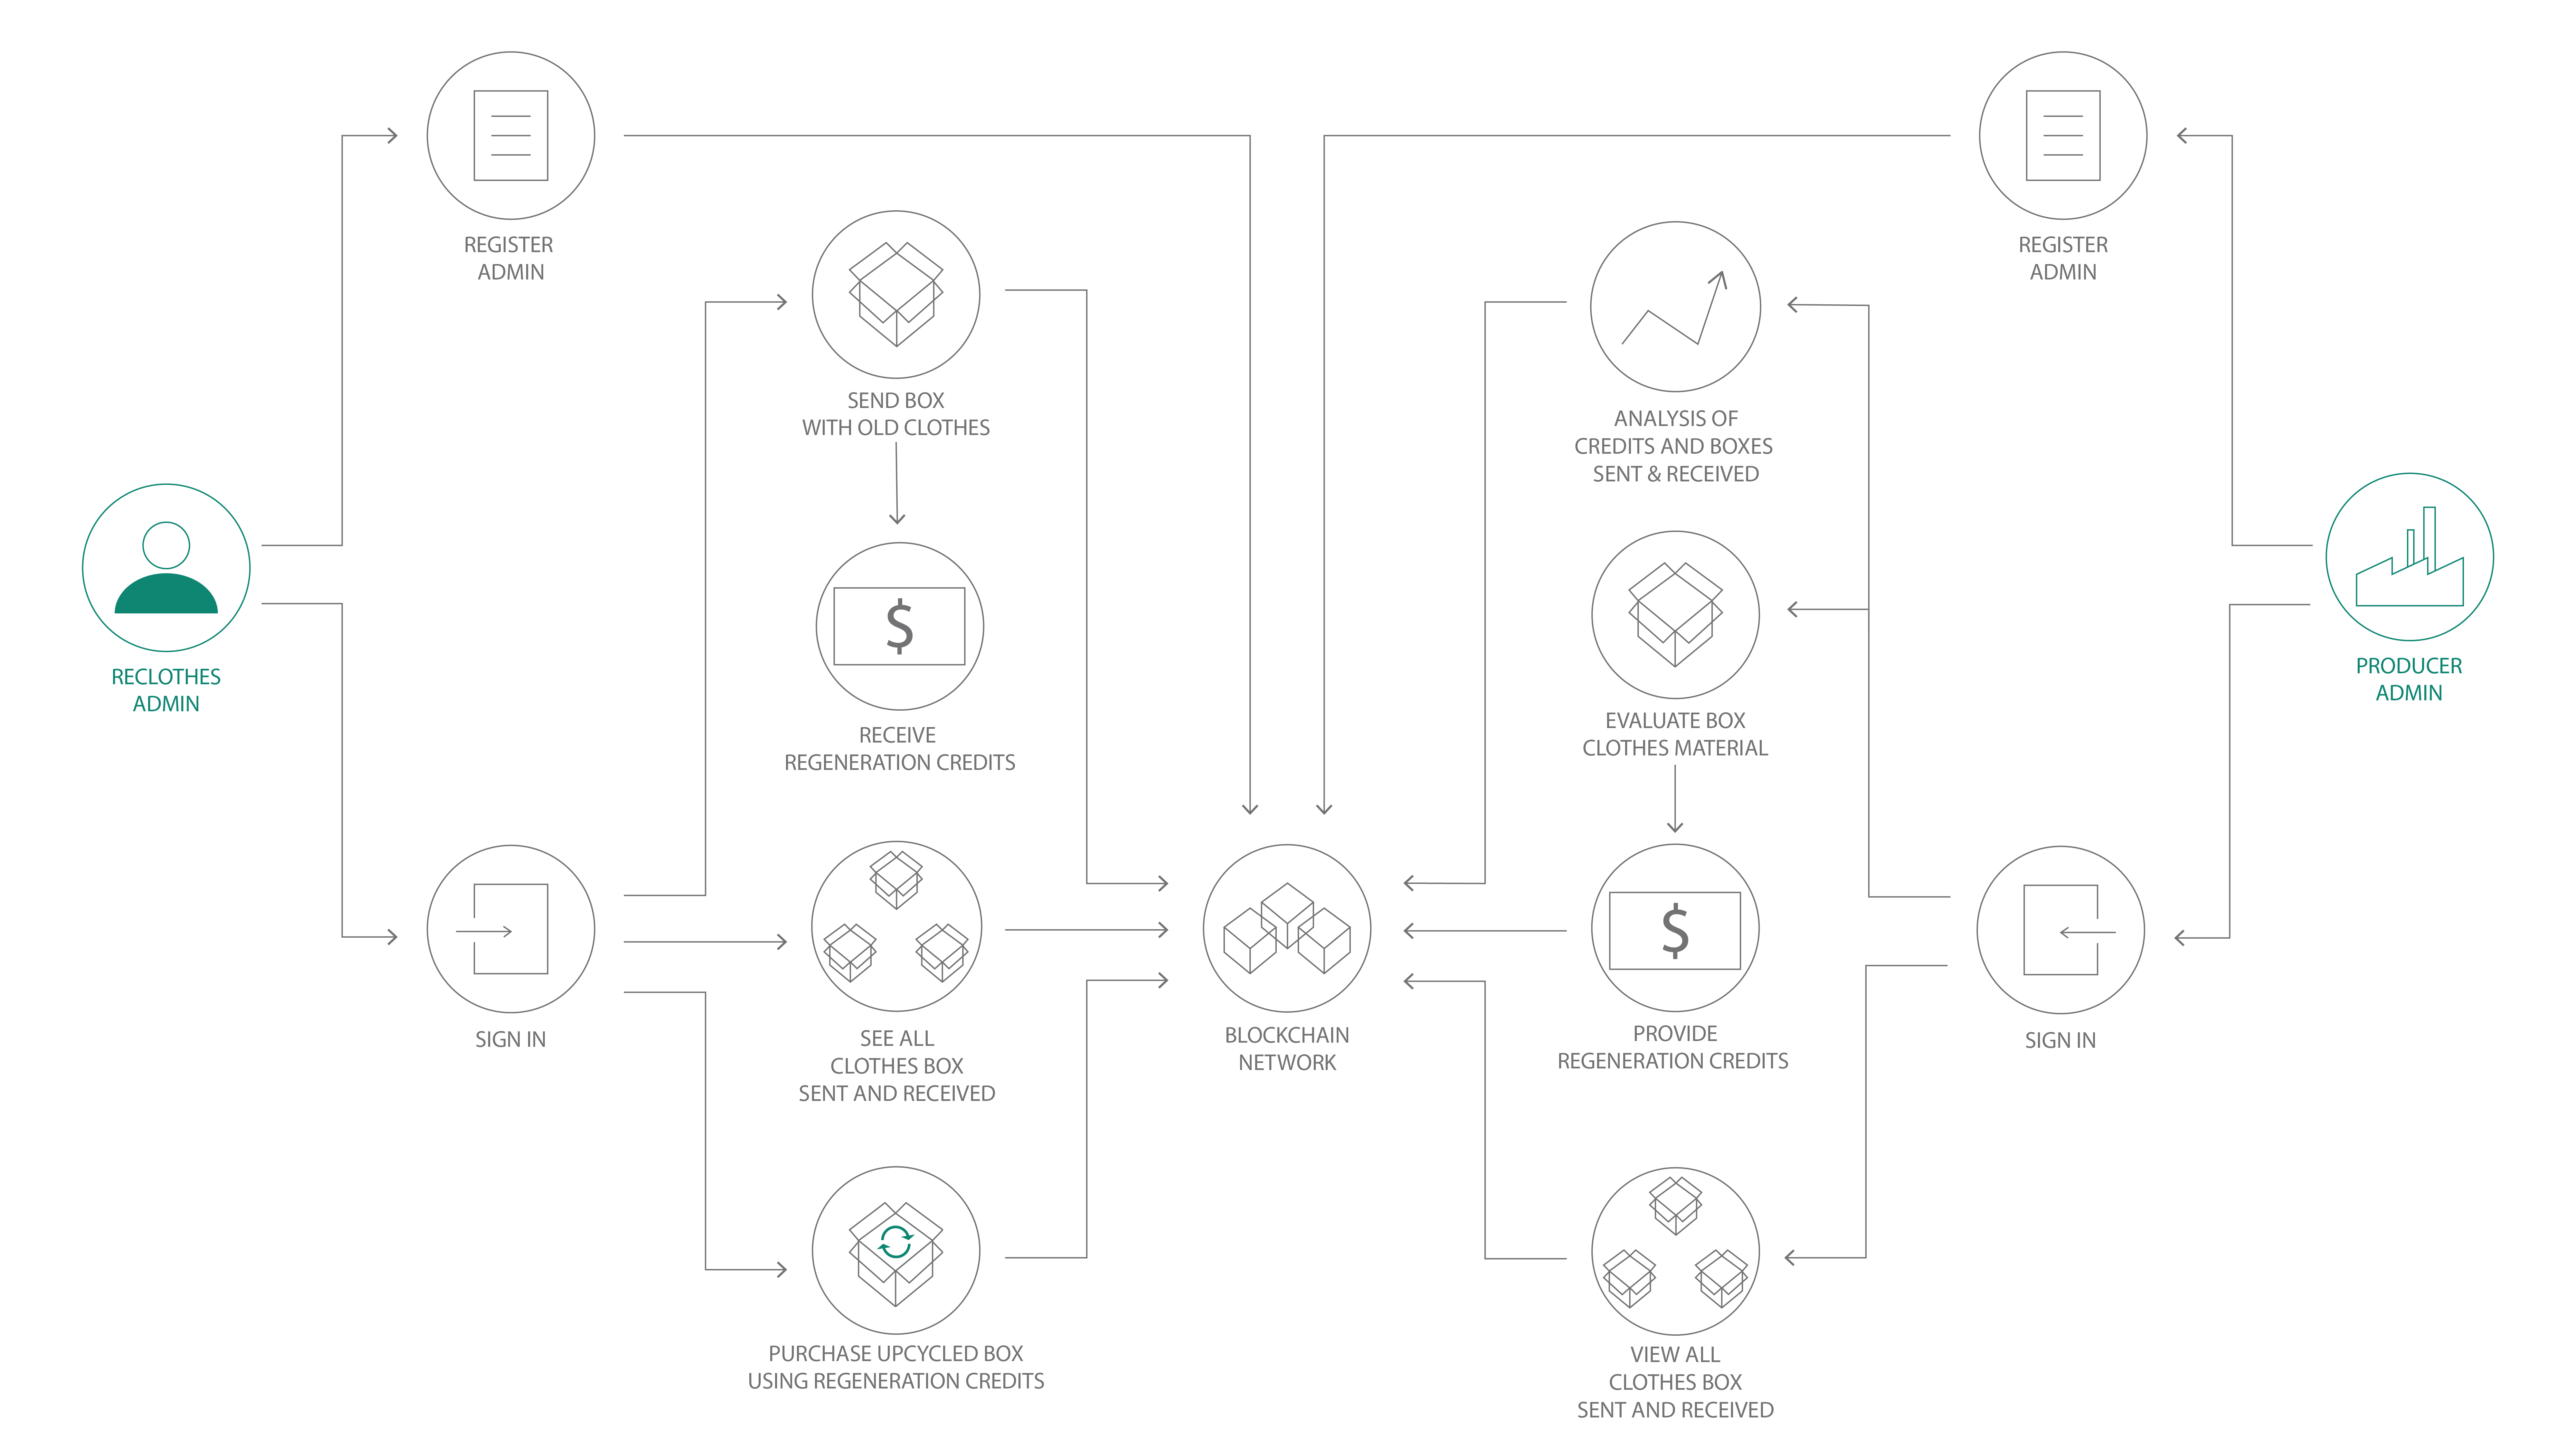
\includegraphics[totalheight=10cm]{img/use_case2.png}
	\caption{UseCase 2}
	\label{fig:usecase2}
\end{figure}


%SMART CONTRACT
\newpage
\section{Smart Contract}

For the smart contract developments we exploit the \texttt{fabric-chaincode-evm}\footnote{To run Solidity Contract over Fabric Network, 
It's used \texttt{fabric-chaincode-evm}, an ethereum virtual machine chaincode developed by IBM developers,
to allow the integrations there's the need of additional components such as Fab3 Proxy}, it allow to run ethereum
smart contract bytecode inside an Hyperledger Fabric peer. Therefore evm chaincode allow us the development
of the smart contract in Solity or Vyper programming languages. 
\bigskip

For the development it's user \textbf{Remix}\footnote{http://remix.ethereum.org/}, It's an online
editor that allow to write and compile Solidity smart contracts code, providing all the Solidity
version compiler. Once that the smart contract code is wrote and the \texttt{.sol} file is produced, 
the compiling process produce two files mandatory for the deployment and use of the smart contract 
over fabric network. 
The two file produced are: 
\begin{outline}
    \1 \textbf{ABI}: The \textit{Application Binary Interface} is the standard way to interact with 
    contracts in the Ethereum ecosystem, both from outside the blockchain and for contract-to-contract 
    interaction. The ABI is a .json file that describes the deployed contract and its functions. 
    It allows us to contextualize the contract and call its functions. In other world 
    The ABI is the description of the contract interface. It contains no code and cannot be run by 
    itself. It's mandatory for smart contract use because the bytecode is the executable EVM code, 
    but by itself it is without context.

    \1 \textbf{Bytecode}: This is the code that is stored on-chain that describes a smart contract. 
    This code does not include the constructor logic or constructor parameters of a contract 
    It's an hexadecimal representation of the final contract. It use the ABI to find the 
    context of the behind contract logic. 
\end{outline}

\bigskip

To handle the overall system was produced three smart contract in Solidity. Two of that run over 
the Hyperledger Fabric network, exploiting the membership mechanism to access of the chaincode.
In other word the permissioned mechanism behind the logic is performed both networks side and 
chaincode side. The network side filter at certificate layer, the access to the network.
On the other hand the registration mechanism implemented over the chaincode filter the user
logged to the network. 
\bigskip

The third smart contract developed run over the Ethereum network, for that project It's used the 
Ropsten testnet. The access to the contract, in this case, is provided by the contract address 
generated during the deployment phase. 
\bigskip

For a better view below we list all the contract involved in the system:
\begin{outline}[enumerate]
    \1 \textbf{Hyperledger Fabric}
    \2 \textbf{User Contract}: handle the the User side, registration and interactions phase. That contract
    shapes the Use Case 1 functionalities. There's the dedicated data structures that cares about storing of actors
    involved( \texttt{User} and \texttt{Admin} ). It provide a set of getter and setter methods and that 
    a couple of function that leads to a transaction process.    
    \2 \textbf{Producer Contract}: handle the interaction from Reclothes to Producers.That contract
    shapes the Use Case 2 functionalities. There's the dedicated data structures that cares about storing of actors
    involved( \texttt{Admin} and \texttt{Producer} ). It provide a set of getter and setter methods and 
    that a couple of function that leads to a transaction process.  

    \1 \textbf{Ethereum}
    \2 \textbf{ERC20 Contract}: it's a standard smart contract with a Max Supply fixed to 1.000.000.
    The contract is stuctured following the ERC20 standard. It's not correlated to this project and
    it's exchangeable amoung user that owns an ethereum wallet. The Contract is deployed over Ropsten network 
    and is accesible using the public contract address. We access to it using an Infura node as Ethereum network endpoint.
\end{outline}

\subsection{User Contract} 

The User Contract contains all the features described in the Hyperledger Fabric part of Use Case 1. 

\subsubsection{Data Structure}

In that contract we are going to store all the transactions informations related to the points and 
clothes box transactions. Moreover we store the informations of the actors involved in the system, that registration 
phase perform an additional control over the actors that are logged in over the Fabric network. The
address specified during the registration phase (\texttt{msg.sender}) is the ethereum address
generated on the fly by Fab3 Proxy. In the following sections there's going to be a better
explanation of Fab proxy module and its use.  
\bigskip

The model of the data structures is divided inside 4 structs:

\begin{outline}[enumerate]
    \1 \textbf{User}: model all users data
    \1 \textbf{Admin}: model Reclothes Admin data
    \1 \textbf{PointsTransaction}: Model transactions data and incorporate \texttt{TransactionType} used to identify the flows
    \1 \textbf{ClothesBox}: The box sent with old clothes 
\end{outline}

\begin{lstlisting}[language=Solidity]
       
    // model a user
        struct User {
            address userAddress;    // User address (inside fabric environment)
            address publicAddress;  // external eth public address of User Admin
            string firstName;
            string lastName;
            string email;
            uint points;            // Fabric points amount
            bool isRegistered;      // Flag for internal use
            uint numTransaction;    // number of transactions performed
            mapping(uint => PointsTransaction) userTransactions;
            uint numBox;            // number of box transaction evaluated
            mapping(uint => ClothesBox) box;
        }
    
        // model a admin
        struct Admin {
            address adminAddress;   // Admin address (inside fabric environment)
            address publicAddress;  // external eth public address of Admin
            string name;
            bool isRegistered;      // Flag for internal use
        }
    
        // model points transaction
        enum TransactionType { Earned, Redeemed }
        struct PointsTransaction {
            uint points;
            TransactionType transactionType;
            address userAddress;    // user address involved
            address adminAddress;   // admin address involved
        }
    
        // model clothes box to ship
        struct ClothesBox {
            address userAddress; // reclothes-producer Admin
            uint tshirt;        // Number of item
            uint pants;         // Number of item
            uint jacket;        // Number of item
            uint other;         // Number of item
            bool isEvaluated;   // Flag to check if box evaluation is performed
            uint points;        // fabric value amount of the box
        }
\end{lstlisting}

\subsubsection{Getter}

The User Contract allow to access to a set of method to obtain informations of the system status.
Once the user is logged in as User or Admin could perform part of that getter invocation.
Parts of the method are developed for an internal usage, the other ones are dedicated
to provide to the actors information about the system, or is usefull to start other invokations
dapp side. The access to some method are handled using modifier method that perform a filtering
process of the function caller. 
\bigskip 

\begin{lstlisting}[language=Solidity]
    
    /***********************************************/
    /***************** Users Data ******************/
    /***********************************************/
    //get User eth public address
    function getUserEthAddress() onlyUser() public view returns(address ethAddress){
        return users[msg.sender].publicAddress;
    }

    //get Reclothes Admin eth public address
    function getAdminEthAddress() onlyAdmin() public view returns(address ethAddress){
        return admins[msg.sender].publicAddress;
    }

    /****************************************************/
    /*** All Box Requests -> Old, Evaluated, UpCycled ***/
    /****************************************************/

    //Get PendingBox by index
    function getPendingRequest(uint _pendingIndex) public view returns(address, uint, uint, uint, uint, bool, uint) {
        // only admin can call
        require(admins[msg.sender].isRegistered, "Admin address not found");

        //check index
        require(_pendingIndex<pendingIndex, "Wrong index");

        return (pendingBox[_pendingIndex].userAddress, pendingBox[_pendingIndex].tshirt, pendingBox[_pendingIndex].pants, pendingBox[_pendingIndex].jacket, pendingBox[_pendingIndex].other, pendingBox[_pendingIndex].isEvaluated, pendingBox[_pendingIndex].points);
    }

    //Get Next Pending Request
    function getNextPendingRequest() onlyAdmin(msg.sender) public view returns(address, uint, uint, uint, uint, bool, uint) {
        //check index
        require(evaluatedIndex<pendingIndex, "No More Pending Request");

        return (pendingBox[evaluatedIndex].userAddress, pendingBox[evaluatedIndex].tshirt, pendingBox[evaluatedIndex].pants, pendingBox[evaluatedIndex].jacket, pendingBox[evaluatedIndex].other, pendingBox[evaluatedIndex].isEvaluated, pendingBox[evaluatedIndex].points);
    }

    //Get EvaluatedBox by index
    function getEvaluatedRequest(uint _evaluatedIndex) public view returns(address, uint, uint, uint, uint, bool, uint) {
        // only admin can call
        require(admins[msg.sender].isRegistered, "Admin address not found");

        //check index
        require(_evaluatedIndex<evaluatedIndex, "Wrong index");

        return (evaluatedBox[_evaluatedIndex].userAddress, evaluatedBox[_evaluatedIndex].tshirt, evaluatedBox[_evaluatedIndex].pants, evaluatedBox[_evaluatedIndex].jacket, evaluatedBox[_evaluatedIndex].other, evaluatedBox[_evaluatedIndex].isEvaluated, evaluatedBox[_evaluatedIndex].points);
    }

    function getTransactionInfo(uint _transactionIndex) onlyUser(msg.sender) public view returns(uint, uint, address, address) {
        //require index exists
        require(users[msg.sender].numTransaction > _transactionIndex && _transactionIndex >= 0, "Wrong transaction index");

        return (users[msg.sender].userTransactions[_transactionIndex].points, uint(users[msg.sender].userTransactions[_transactionIndex].transactionType), users[msg.sender].userTransactions[_transactionIndex].userAddress, users[msg.sender].userTransactions[_transactionIndex].adminAddress);
    }

    //return box requests number
    function getUserBoxNum() onlyUser(msg.sender) public view returns(uint) {
        return users[msg.sender].numBox;
    }

    //Get UserBox by index
    function getUserRequest(uint _index) onlyUser(msg.sender) public view returns(address, uint, uint, uint, uint, bool, uint) {
        //check index
        require(_index<users[msg.sender].numBox, "Wrong index");

        ClothesBox memory box = users[msg.sender].box[_index];

        return (box.userAddress, box.tshirt, box.pants, box.jacket, box.other, box.isEvaluated, box.points);
    }

    function getAdminTransactionInfo(uint _transactionIndex) onlyAdmin(msg.sender) public view returns(uint, uint, address, address) {
        //require index exists
        require(totTx > _transactionIndex && _transactionIndex >= 0, "Wrong transaction index");

        return (usersTransactions[_transactionIndex].points, uint(usersTransactions[_transactionIndex].transactionType), usersTransactions[_transactionIndex].userAddress, usersTransactions[_transactionIndex].adminAddress);
    }

    //return tot transaction number
    function getTotTransactionNum() onlyAdmin(msg.sender) public view returns(uint) {
        return totTx;
    }

\end{lstlisting}

\subsubsection{Transactions}

The transactions process are the main process of the overall smart contract. That method perform a
write access to the smart contract and going to be to modify the world state of the ledger
stored over the Fabric blockchains peers. 
\bigskip 

There's two functions that performs transactions between actors involved in the smart contracts,
these are :

\begin{outline}[enumerate]
    \1 \textbf{earnPoints}: It's an internal function called by \texttt{EvaluateBox} function.
    Once that user performed the \texttt{sendBox} process, start the evaluation process, Admin side.
    Therefore the admin evaluate the pending request and set a total amount of points related to 
    the box received. That the \texttt{EvaluateBox} function call the internal function \texttt{earnPoints}
     passing as argument the amount to be transfer and the userAddress of the clothes box sender. Than
     the function performs the fabric points transaction from Reclothes to User.
    
     \1 \textbf{usePoints}: It's related to the purchase process. When the User perform a purchase over
     the platform store, there's be calculated the overall amount related to the items purchased and internally
     is invoked the \texttt{usePoints} function. That function after a set of previous checks than going to 
     decrease the user balance of the related amount passed to the function.
\end{outline}

\begin{lstlisting}[language=Solidity]
    
    /****************************************************/
    /************* Transactions Operations **************/
    /****************************************************/

    //update users with points earned
    function earnPoints (uint _points, address _userAddress ) onlyAdmin(msg.sender) internal {

      // verify user address
      require(users[_userAddress].isRegistered, "User address not found");

      // update user account
      users[_userAddress].points = users[_userAddress].points + _points;

      PointsTransaction memory earnTx = PointsTransaction({
        points: _points,
        transactionType: TransactionType.Earned,
        userAddress: _userAddress,
        adminAddress: admins[msg.sender].adminAddress
      });

      // add transction
      transactionsInfo.push(earnTx);

      users[_userAddress].userTransactions[users[_userAddress].numTransaction] = earnTx;
      users[_userAddress].numTransaction++;

      usersTransactions[totTx] = earnTx;
      totTx++;

    }

    //Update users with points used
    function usePoints (uint _points) onlyUser(msg.sender) public {

      // verify enough points for user
      require(users[msg.sender].points >= _points, "Insufficient points");

      // update user account
      users[msg.sender].points = users[msg.sender].points - _points;

      PointsTransaction memory spendTx = PointsTransaction({
        points: _points,
        transactionType: TransactionType.Redeemed,
        userAddress: users[msg.sender].userAddress,
        adminAddress: 0
      });

      // add transction
      transactionsInfo.push(spendTx);

      users[msg.sender].userTransactions[users[msg.sender].numTransaction] = spendTx;
      users[msg.sender].numTransaction++;

      usersTransactions[totTx] = spendTx;
      totTx++;
    }

    /****************************************************/
    /************** Clothes Box Operations **************/
    /****************************************************/

    //handle box
    function sendBox(uint _tshirt, uint _pants, uint _jackets, uint _other) onlyUser(msg.sender) public {

         pendingBox[pendingIndex] = ClothesBox({
             userAddress: msg.sender,
             tshirt: _tshirt,
             pants: _pants,
             jacket: _jackets,
             other: _other,
             isEvaluated: false,
             points: 0
         });

         users[msg.sender].box[users[msg.sender].numBox] = pendingBox[pendingIndex];

         users[msg.sender].numBox++;
         pendingIndex++;
    }

    //evaluate box
    function evaluateBox(uint _points) onlyAdmin(msg.sender) public {
        //check correct pending request index
        require(evaluatedIndex < pendingIndex, "No more pending request");

        //check if evaluation is done
        require(!pendingBox[evaluatedIndex].isEvaluated, "Request just evaluated");

        //pop pending request
        ClothesBox storage box = pendingBox[evaluatedIndex];

        //update box transaction
        box.isEvaluated = true;
        box.points = _points;

        //send points to the userAddress
        earnPoints(_points, box.userAddress);

        //add evaluated box
        evaluatedBox[evaluatedIndex] = box;
        evaluatedIndex++;
    }

    //get user balance
    function getBalance() public view returns (uint) {
        return users[msg.sender].points;
    }
\end{lstlisting}

%% producer contract 
\subsection{Producer Contract}

The Producer Contract contains all the features described in the Use Case 2 diagram shown in 
the Figure \ref{fig:usecase2}.

\subsubsection{Data Structure}

In that contract we are going to store all the transactions informations related to the points and 
clothes box transactions. Moreover we store the informations of the actors involved in the system, in
this case the actors involed going to be \texttt{Admin} and \texttt{Producer}.
As the previous contract the registration phase provide an additional control over the actors logged 
in over the Fabric network. The address specified during the registration phase (\texttt{msg.sender}) is 
the ethereum address generated on the fly by Fab3 Proxy. 
\bigskip

Briefly explaing the behaviour of relationship amoung contracts,  the fab proxy has a 1 to 1 association 
instance/user. There's the possibility that the Admin logged and registered, over \texttt{UserContract}, associated to one fab3 instance, setted over the channel that communicate with 
\texttt{UserContract}, must to perform another registration with a new fab3 proxy instance
setted to communicate with the channel dedicated for \texttt{ProducerContract}. It means that for each
fab3 instance there's be a new eth address generated and the Admin could has two ethereum address,
one associated to \texttt{UserContract} and the other one associated to \texttt{PrducerContract}.
\bigskip


The model of the data structures is divided inside 3 structs:

\begin{outline}[enumerate]
    \1 \textbf{Producer}: model all producers data
    \1 \textbf{Admin}: model Reclothes Admin data
    \1 \textbf{ClothesBox}: The box sent with old clothes 
\end{outline}

\begin{lstlisting}[language=Solidity]
    // model a producer
    struct Producer {
        address adminAddress;   // Producer Admin address (inside fabric environment)
        address publicAddress;  // external eth public address of Producer Admin
        string name;            // Producer admin name
        bool isRegistered;      // Flag for internal use
        uint numBox;            // number of box transactions evaluated
        uint pointsProvided;    // amount of points provided by own evaluations
        mapping(uint => ClothesBox) box;
    }

    // model a admin
    struct Admin {
        address adminAddress;   // Admin address (inside fabric environment)
        address publicAddress;  // external eth public address of Admin
        string name;            // Admin name
        bool isRegistered;      // Flag for internal use
        uint numBox;            // number of box transaction evaluated
        uint creditSpent;       // amount of points provided by own evaluations
        mapping(uint => ClothesBox) box;
    }

    struct ClothesBox {
        address adminAddress; // reclothes-producer Admin
        uint tshirt;        // Number of item
        uint pants;         // Number of item
        uint jacket;        // Number of item
        uint other;         // Number of item
        bool isEvaluated;   // Flag to check if box evaluation is performed
        uint points;        // fabric value amount of the box

        //mapping(uint => Clothes) clothes;
    }
\end{lstlisting}

\subsubsection{Getter}

The Producer Contract allow to access to a set of method to obtain informations of the system status.
Once the user is logged in as Admin or Producer could perform part of that getter invocation.
Parts of the method are developed for an internal usage, the other ones are dedicated
to provide to the actors information about the system, or is usefull to start other invokations
dapp side. The access to some method are handled using modifier method that perform a filtering
process of the function caller. 
\bigskip 

Below I reported only the main smart contract methods.
\bigskip

\begin{lstlisting}[language=Solidity]
   
    /****************************************************/
    /*** All Box Requests -> Old, Evaluated, UpCycled ***/
    /****************************************************/

    function getPendingRequest(uint _pendingIndex) public view returns(address, uint, uint, uint, uint, bool, uint) {
        //check index
        require(_pendingIndex<pendingIndex && _pendingIndex>=0, "Wrong index");

        return (pendingBox[_pendingIndex].adminAddress, pendingBox[_pendingIndex].tshirt, pendingBox[_pendingIndex].pants, pendingBox[_pendingIndex].jacket, pendingBox[_pendingIndex].other, pendingBox[_pendingIndex].isEvaluated, pendingBox[_pendingIndex].points);
    }

    function getNextPendingRequest() public view returns(address, uint, uint, uint, uint, bool, uint) {
        //check index
        require(evaluatedIndex<pendingIndex, "No More Pending Request");

        return (pendingBox[evaluatedIndex].adminAddress, pendingBox[evaluatedIndex].tshirt, pendingBox[evaluatedIndex].pants, pendingBox[evaluatedIndex].jacket, pendingBox[evaluatedIndex].other, pendingBox[evaluatedIndex].isEvaluated, pendingBox[evaluatedIndex].points);
    }


    /********* Evaluated Request -> Box with Old Clothes evaluated *********/
    function getEvaluatedRequest(uint _evaluatedIndex) public view returns(address, uint, uint, uint, uint, bool, uint) {
        //check index
        require(_evaluatedIndex<evaluatedIndex && upCycledIndex>=0, "Wrong index");

        return (evaluatedBox[_evaluatedIndex].adminAddress, evaluatedBox[_evaluatedIndex].tshirt, evaluatedBox[_evaluatedIndex].pants, evaluatedBox[_evaluatedIndex].jacket, evaluatedBox[_evaluatedIndex].other, evaluatedBox[_evaluatedIndex].isEvaluated, evaluatedBox[_evaluatedIndex].points);
    }


    /********* UpCycled Request -> Box with New Clothes *********/
    function getUpCycledRequest(uint _upCycledIndex) public view returns(address, uint, uint, uint, uint, bool, uint) {
        //check index
        require(_upCycledIndex<upCycledIndex && upCycledIndex>=0, "Wrong index");

        return (upCycledBox[_upCycledIndex].adminAddress, upCycledBox[_upCycledIndex].tshirt, upCycledBox[_upCycledIndex].pants, upCycledBox[_upCycledIndex].jacket, upCycledBox[_upCycledIndex].other, upCycledBox[_upCycledIndex].isEvaluated, upCycledBox[_upCycledIndex].points);
    }

    /****************************************************/
    /***************** Data of Requests *****************/
    /****************************************************/

    function getTotPointsProvided() public view returns(uint) {
        return totPointsProvided;
    }

    function getRegenerationCredit() public view returns(uint) {
        return debtPoints;
    }

    function getTotBoxOld() public view returns(uint) {
        return totBoxOld;
    }

    function getTotBoxNew() public view returns(uint) {
        return totBoxNew;
    }

\end{lstlisting}

\subsubsection{Transactions}

As always be the transactions process are the main ones of the smart contrancts, leadind to a write
operation.
\bigskip.

There's two functions that perform transactions between the actors involved in that contract:

\begin{outline}[enumerate]
    \1 \textbf{evaluateBox}: The evaluation process start by the invocation of \texttt{SendBox} function.
    Once that there's pending box request, the next one going to be evaluated and following
    the price table, to evaluate clothes materials by \texttt{material type} and \texttt{weight},
    there's setted an overall amount value corresponding to the clothes box request.
    The transfer process, considering just one Producer involved in own project, so the points is 
    handled with a \texttt{debtPoints} variable that is updated by these two functions. In that
    case \texttt{evaluateBox} going to add the amount value of the box to that \texttt{debtPoints} variable. 

    \1 \textbf{buyUpcycledBox}: That process leads a purchase order performed by the Admin to the 
    Producer. Admin choose a kind of fixed box(\texttt{small, medium, large}) with a fixed Regeneration
    Credits price associated. Before performing the purchase process, It's checked the \texttt{debtPoints}
    balance to allow or not the transaction of the box. Once that the amount of regeneration credits
    is enough to buy upcycled clothes, than the \texttt{debtPoints} is updated and the value of the
    purchased box is subtract to the overall balance. 
\end{outline}

\begin{lstlisting}[language=Solidity]
    
    // Evaluate Old Box
    function evaluateBox(uint _points) onlyProducer() public {
        //check correct pending request index
        require(evaluatedIndex < pendingIndex, "No more pending request");

        //check if evaluation is done
        require(!pendingBox[evaluatedIndex].isEvaluated, "Request just evaluated");

        //pop pending request
        ClothesBox storage box = pendingBox[evaluatedIndex];

        //update box transaction
        box.isEvaluated = true;
        box.points = _points;

        //add evaluated box
        evaluatedBox[evaluatedIndex] = box;
        evaluatedIndex++;

        debtPoints += _points;
        totPointsProvided += _points;
    }

    function buyUpcycledBox(uint _tshirt, uint _pants, uint _jackets, uint _other, uint _points) onlyAdmin() public {
        require(debtPoints >= _points, "Not enought credits accumulated in old material boxes");

        ClothesBox memory box = ClothesBox({
         adminAddress: msg.sender,
         tshirt: _tshirt,
         pants: _pants,
         jacket: _jackets,
         other: _other,
         isEvaluated: true,
         points: _points
        });

        admins[msg.sender].box[admins[msg.sender].numBox] = box;
        admins[msg.sender].numBox++;
        admins[msg.sender].creditSpent += _points;

        //add upcycled box
        upCycledBox[upCycledIndex] = box;
        upCycledIndex++;

        debtPoints -= _points;
        totBoxNew++;
    }

\end{lstlisting}

%% erc20 contract
\subsection{ERC20 Contract}
\label{erc20}

ERC-20 is a technical standard used to issue and implement tokens on the Ethereum blockchain
The standard describes a common set of rules that should be followed for a token to function properly
 within the Ethereum ecosystem. Therefore, ERC-20 should not be considered as a piece of code or 
 software. Instead, it may be described as a technical guideline or specification.
\bigskip

The choose to develop an ERC-20 token leads to relaxing the limitation related to the token
usage. That contract is deployed over the Ethereum network and it's public, accessible to everyone
that own an ethereum wallet. The decision as well as a cross-chain interaction process, lead to 
open the doors to an exteral usage of the token, due to what the asset represents.
\bigskip

The asset want to represent the CO\textsubscript{2} emission saved. For example as asset exchange to
measure the emission saved recycling a tshirt even to produce it starting from scratch.
\bigskip

The main information associated to the created token are: 

\begin{outline}
    \1 \textbf{Symbol}: CO2, It's used to identify a token, this is a three or four letter abbreviation of the token.
    \1 \textbf{Name}: CarbonToken, are able to identify them.
    \1 \textbf{Total supply}: 100000000, It's the max sullpy of the token.
    \1 \textbf{Decimals}: 18, It's used to determine to what decimal place the amount of the token will be calculated. 
    The most common number of decimals to consider is 18. 
\end{outline}

The main features of the contract are describer by ERC20 interface

\begin{lstlisting}[language=Solidity]
    contract ERC20Interface {
        function totalSupply() public constant returns (uint);
        function balanceOf(address tokenOwner) public constant returns (uint balance);
        function allowance(address tokenOwner, address spender) public constant returns (uint remaining);
        function transfer(address to, uint tokens) public returns (bool success);
        function approve(address spender, uint tokens) public returns (bool success);
        function transferFrom(address from, address to, uint tokens) public returns (bool success);
    
        event Transfer(address indexed from, address indexed to, uint tokens);
        event Approval(address indexed tokenOwner, address indexed spender, uint tokens);
    }
\end{lstlisting}

\bigskip

Below I list and explain in details the six mandatory functions that defines the erc20 tokens:

\begin{outline}
    \1 \textbf{totalSupply()}: the supply could easily be fixed, as it is with Bitcoin, this function 
    allows an instance of the contract to calculate and return the total amount of the token that exists 
    in circulation.
    \1 \textbf{balanceOf()}: This function allows a smart contract to store and return the balance of 
    the provided address. The function accepts an address as a parameter, so it should be known that 
    the balance of any address is public.
    \1 \textbf{approve()}: When calling this function, the owner of the contract authorizes, or approves, 
    the given address to withdraw instances of the token from the owner’s address.
    \1 \textbf{transfer()}: This function lets the owner of the contract send a given amount of the token 
    to another address just like a conventional cryptocurrency transaction.
    \1 \textbf{transferFrom()}: This function allows a smart contract to automate the transfer process 
    and send a given amount of the token on behalf of the owner.
    \1 \textbf{allowance()}: This functions allow the caller to check if the given balance's address has 
    enough token to send the amount to an other address.
\end{outline}

% NETWORK
\newpage
\section{Network Architecture}

\subsection{Main Components}

Before to going deeper to explain my network architectural choice is important to have an overview
of the principal components involved in the Hyperledger Fabric Architecture:

\begin{outline}[enumerate]
    \1 \textbf{Peer}: It's the fabric node, there's differt tipe of peers and each of that could perform
    specific actions
    \2 \textbf{Anchor Peer}: this kind of peer is used for communications between organizations. It makes peers in different organizations aware each other.
    \2 \textbf{Committing Peer}: Every peer in the channel
    \2 \textbf{Endorsing Peer}: every peer that has the smart contract installed can be an endorsing peer.
    \2 \textbf{Peer Node}: each peer mantains a copy of the ledger for each channel it is a member of.
    \2 \textbf{Leader Peer}: an organization can have multiple peers ina channel. Only one peer from the organization needs to receive the transactions. The leader distributes transactiond from orderers    
    \1 \textbf{Certification Authority}: Everyone who wants to interact with the network needs an identity. The CA provides the means for each actor to have a verificable digital identity, thanks to that is implemented the membership mechanism providing a permissioned blockchain. 
    \1 \textbf{MSP}: Membership Service Providers (MSP) is a Hyperledger Fabric component that offers an abstraction of membership operations. In particular, an MSP abstracts away all cryptographic mechanisms and protocols behind issuing certificates, validating certificates, and user authentication.
    \1 \textbf{Orderer}: Is like a network administration point. The ordering nodes support the application channels for ordering transactions, create blocks and add it to the chain.  
    \1 \textbf{Organization}: Identify a category of users involved in the network. each user certificate of the Organizations are released by the same CA. The organizations are used in permissioned mechanism allowing or not read and write access to specific data over the network.
    \1 \textbf{Consortium}: A group of organizations that share a need to transact. It could share a set of permission over the network.
    \1 \textbf{Channel}: A channel allow a consortium, group of partecipants, to create a separate ledger of transactions. The transactions, stored in the world state, are visible only to the members of the channel.
    \1 \textbf{Ledger}: It is stored over the peer and consiste to the Worls State of the blockchains. All the transactions performed over the chain is merkled in the world state\footnote{https://en.wikipedia.org/wiki/Merkle_tree}
\end{outline}


\subsection{Own Architecure}

The \textbf{Figure \ref{fig:fabric_network}} show the main components of own network architecture 
build for the application. It includes:

\begin{outline}[enumerate]
    \1 \textbf{3 Peer}: One dedicated peer for each organization involved in the system. 

    \1 \textbf{1 Orderer} organization with \textit{1 ordered} node running

    \1 \textbf{3 Organizations} each with 1 peer, Peer0, running
    \2 \textit{Org1}: User Organization
    \2 \textit{Org2}: Reclothes Admin Organization 
    \2 \textit{Org3}: Producer Organization

    \1 \textbf{2 Channels}
    \2 \textit{Chanel12}: It's the cannel between Org1 and Org2 and allow the comunication between User and Reclothes
    \2 \textit{Chanel23}: It's the cannel between Org2 and Org3 and allow the comunication between Reclothes and Producer

    \1 \textbf{2 Consortiums}
    \1 \textbf{CC12}: related to the channel 1, allow the use of actors owned by Org1 and Org2.
    \1 \textbf{CC23}: related to the channel 2, allow the use of actors owned by Org2 and Org3.
\end{outline}

\bigskip
This is a test network, light for test the entire project. Hyperledger Fabric allow to implements in an easy way more components adding
orderer or Peers, it make hyperledger architecture highly modular. For production the architecture needs some modification.
Adding more orderers and peers for each organizations, in order to maximize the fault tolerance.   

\begin{figure}[h!]
	\centering
	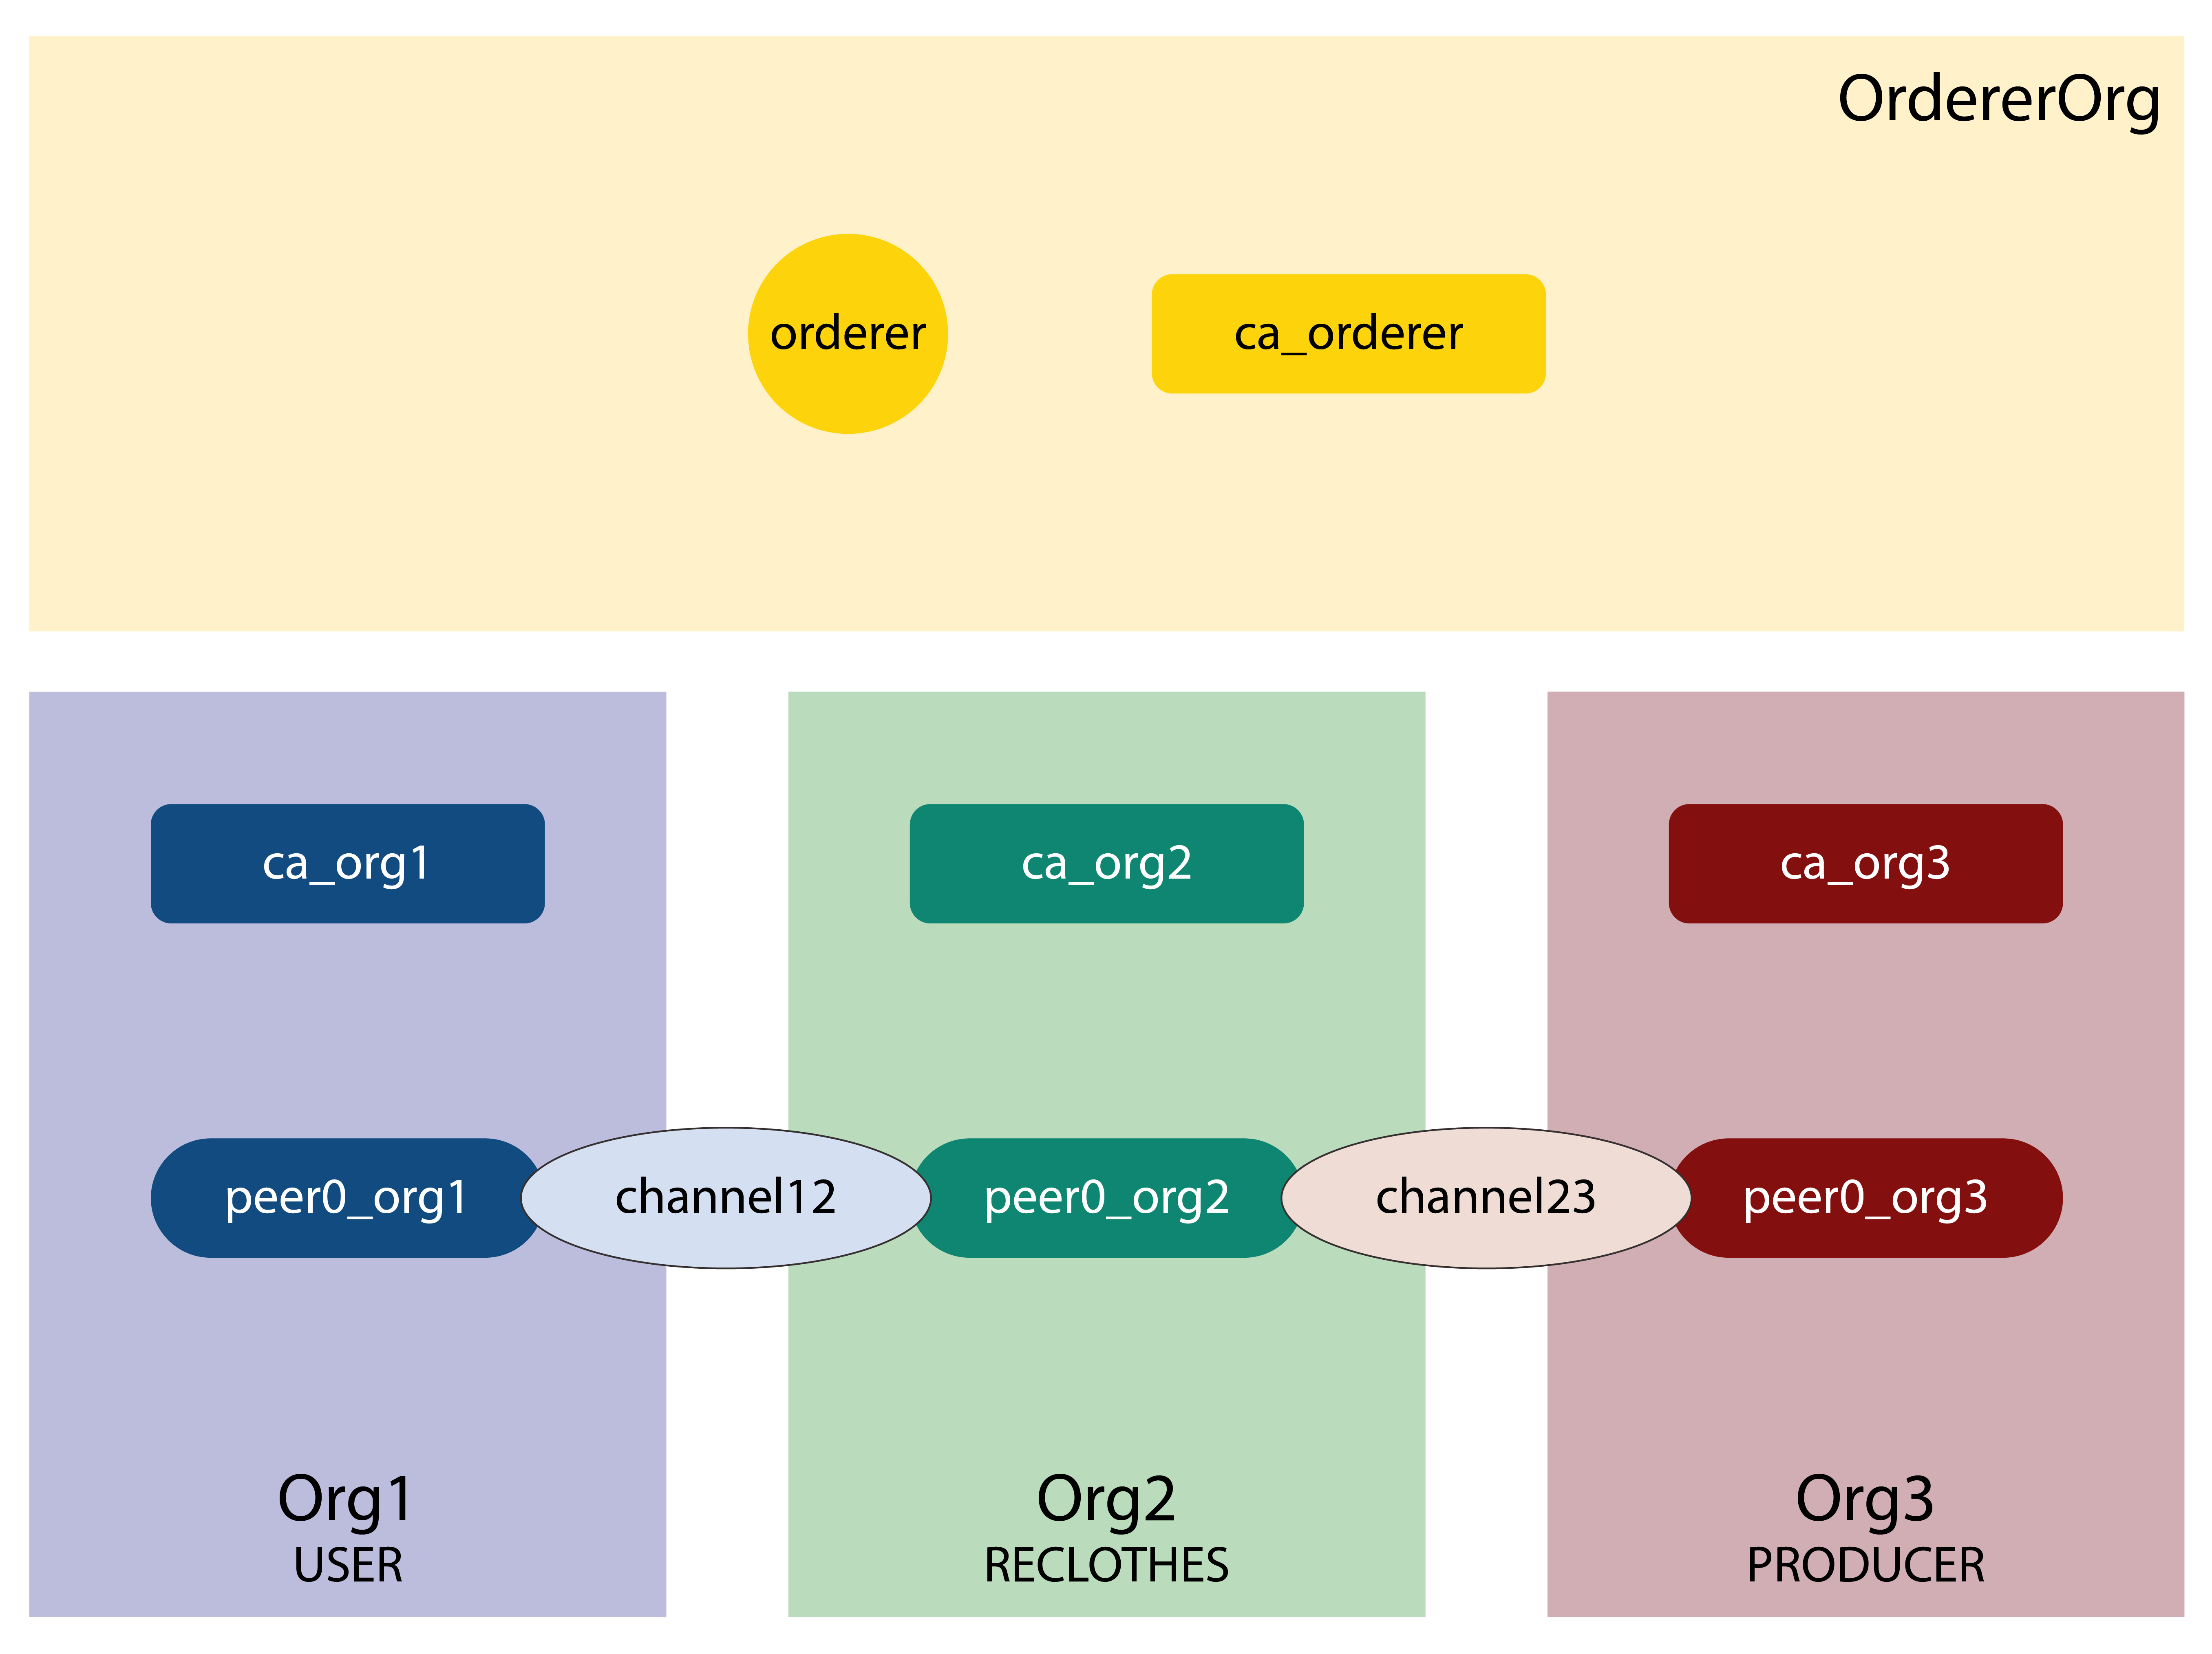
\includegraphics[totalheight=10cm]{img/fabric_network.png}
	\caption{Fabric Network}
	\label{fig:fabric_network}
\end{figure}

\subsection{Fabric Network}

The \textbf{Figure \ref{fig:network}} show how components interact each other. We could separate components into 2 categories,
inside and outside Fabric Network. First of all we need to describe the components involved :

\begin{outline}
    \1 \textbf{Web3 App}: It's the Dapp and the Client connection to the network
    \1 \textbf{Channel}: It's the channel above which transfert data 
    \1 \textbf{CA}: It's the Certification Authority in charge of release certificates.
    \1 \textbf{Peer}: It's "Fabric node", the endpoint of the internal network. It own by specific CA with 
    fixed permissions, linked to the connected channels. 
    \1 \textbf{evm SC}: It's the Ethereum Virtual Machine Chaicode, used to run Solidity Smart Contract. The chaincode 
    is installed over the peer.
    \1 \textbf{ledger}: It's the ledger associated to the channel connected. There's a 1 to 1 association 
    between ledger and channel.
    \1 \textbf{CC}: It's the \textit{Consortium}, It's associated to the channel, manage ownerships and 
    It include a set of Organizations allowed. 
    \1 \textbf{Docker}: The network components run inside docker containers. 
\end{outline}

\begin{figure}[h!]
	\centering
	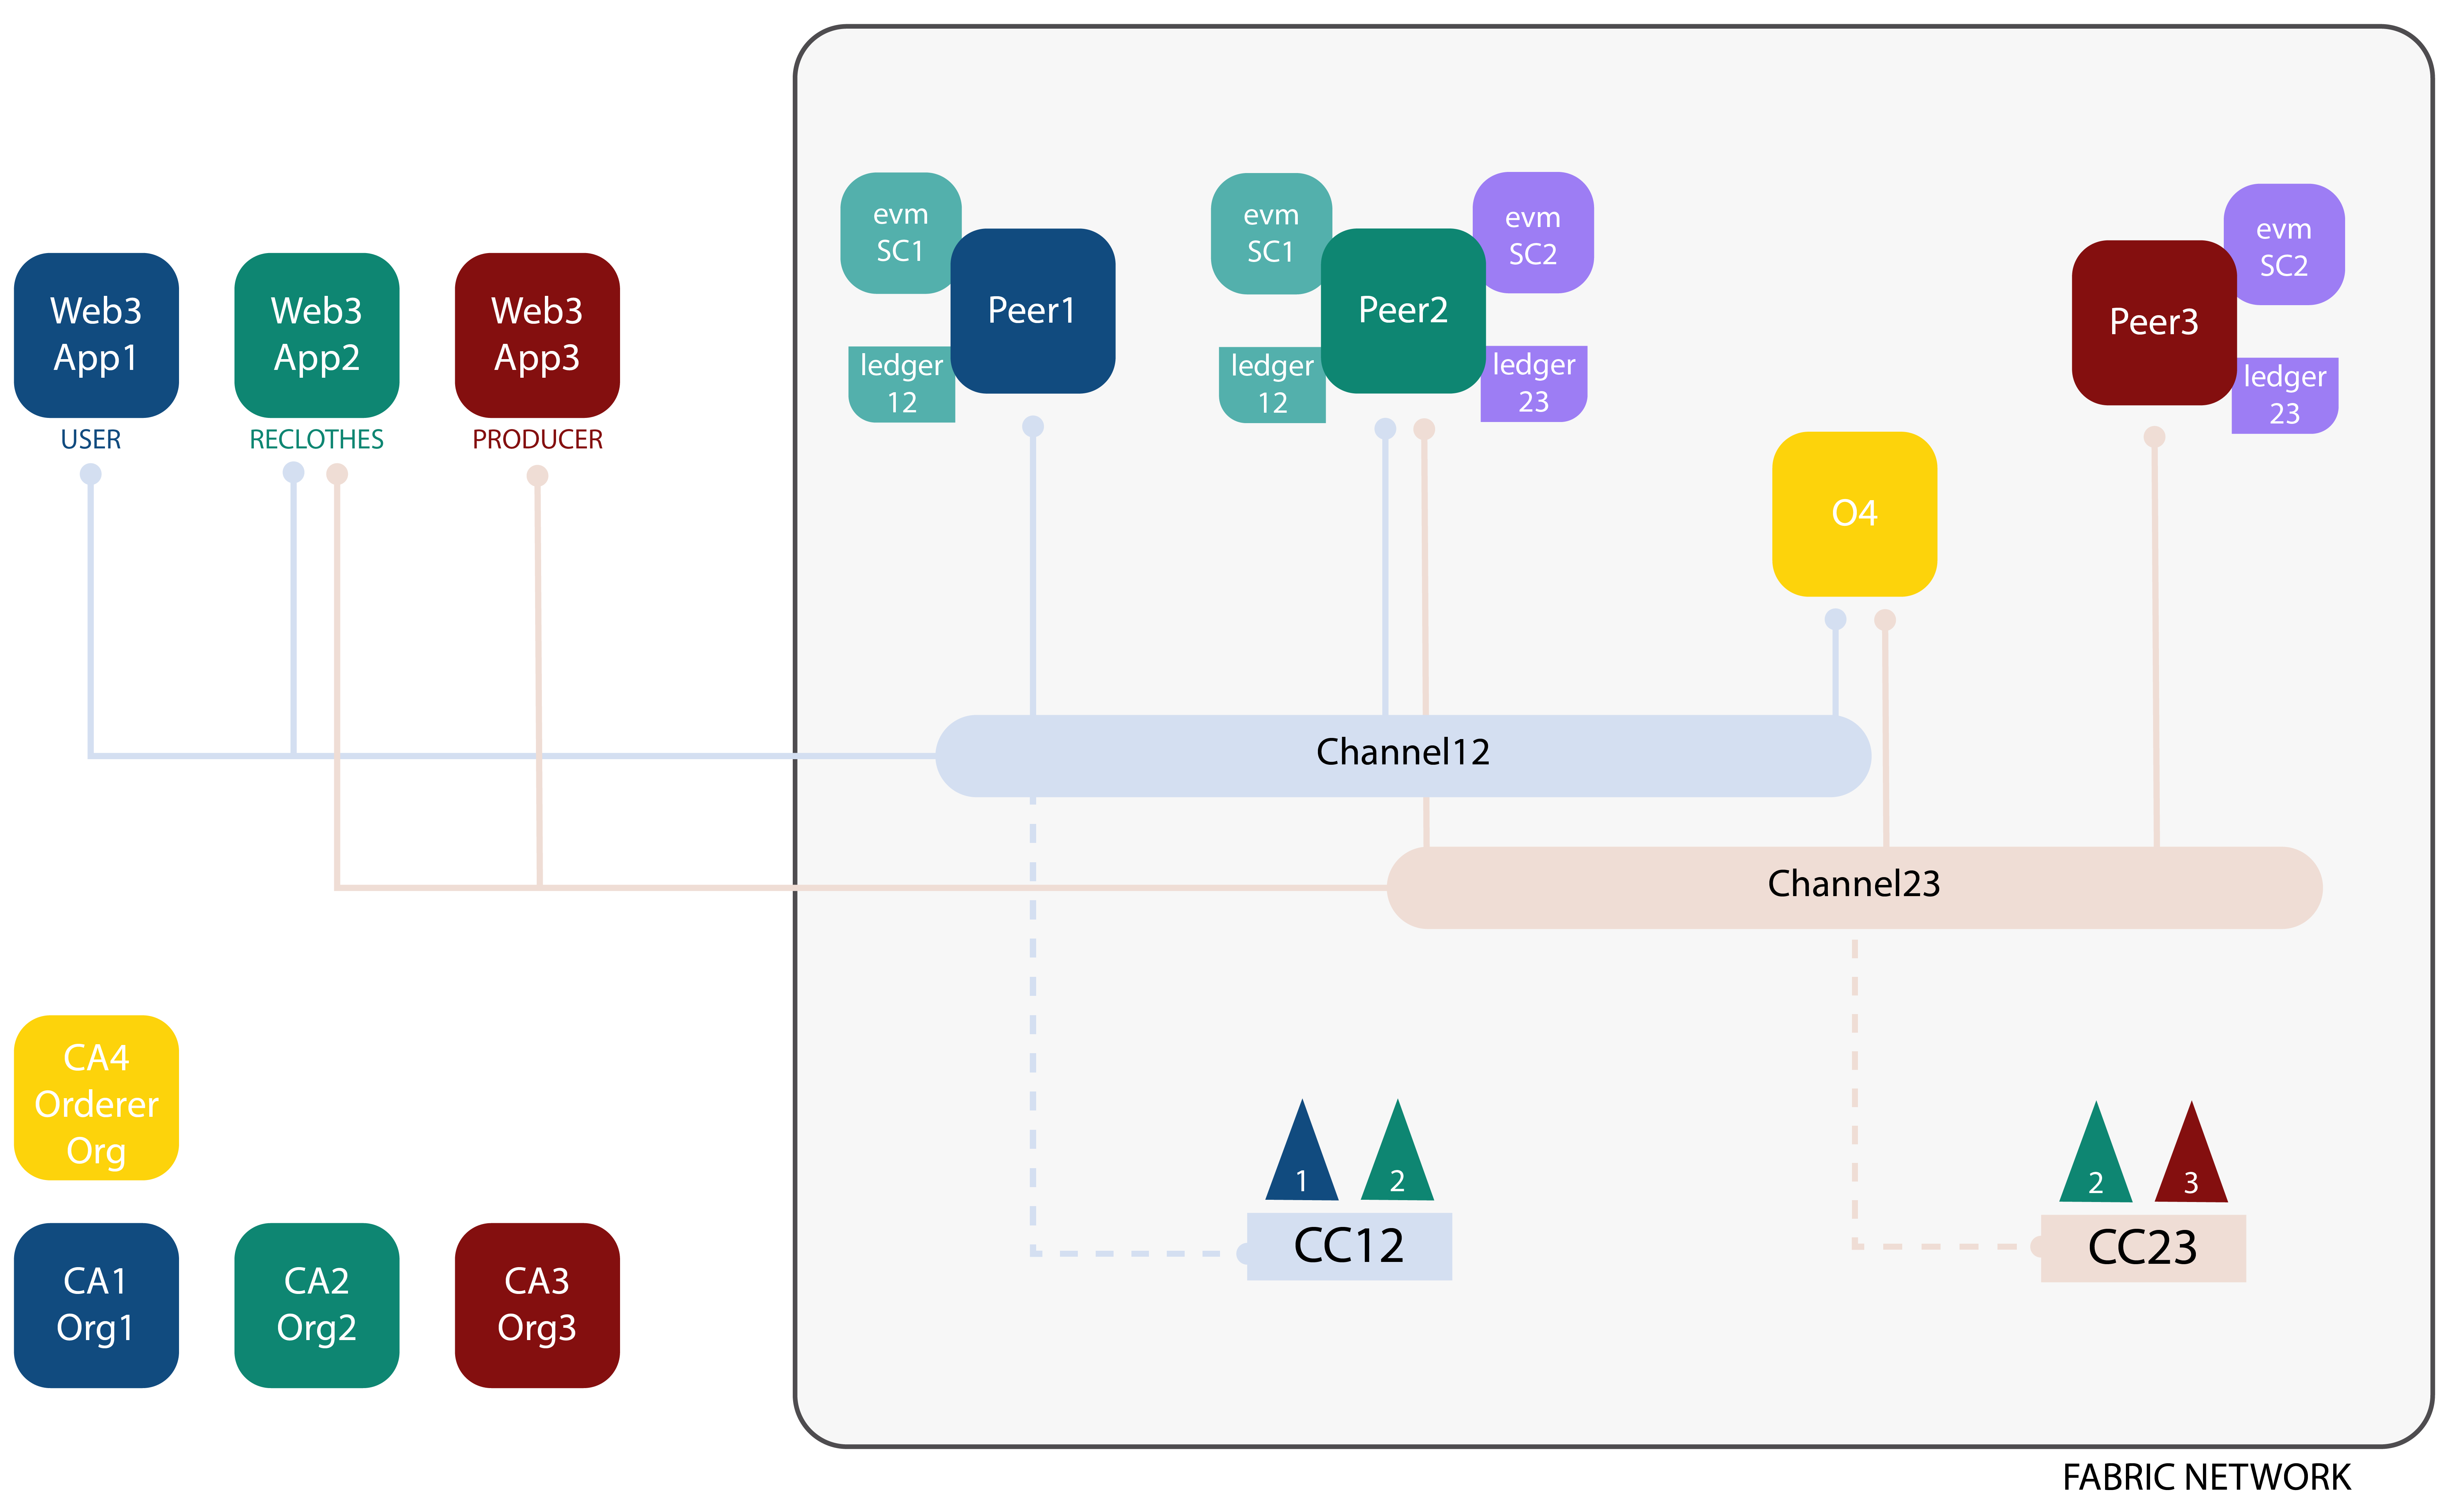
\includegraphics[totalheight=10cm]{img/network.png}
	\caption{Fabric Network Components}
	\label{fig:network}
\end{figure}

By the Figure \ref{fig:network} it's possible to see that in own architecture ther's two ledger, each of that associated
to one channel that involves just part of organizations per channel. The ledger is associated to one or more smart contract 
deployed over the chaincode, in own case we use 1 smart contract deployed each chaincode. 

The \textit{chaincode} is invoked calling the evm chaincode by the \textit{App} Client, using the channel communication.
The channel is the only communication way between external and internal network. The external actor that invoke the chaincode
must to have the priviledges for join to the specified channel. 
The chaincode installed over the peer once is invoked agreed to the request and invoke the chaincode("smart contract")
method. 

Once the method returns, the chaincode forward the reply to the App client. Than the Dapp forward the
answer to the \textit{Orderer} peer that validate the response, create a new block, add it to the chain,
communicate it to the peer in order to syncronize the network and updating the Ledger World State.

\subsubsection{Config File}

Network Architecture in Hyperledger Fabric is highly modular and scalable. Hyperledger provide to the developers a set of developed 
test network\footnote{https://github.com/hyperledger/fabric-samples} for testing purpose and that help developers to understand better 
the structure and the creations steps. The \texttt{fabric-samples} contains a set of tools that allow to release all the cryptographic
materials required for the networks usage, such as certificates related to the user belonging to a specific organization.
In other words all the MSP works is handled by fabric-samples tools. 
\bigskip

The most usefull thing about the hyperledger network is that the components could be added or removed in an easy way.
To design and set up network components and rules, It's wrote the \texttt{config.yaml} file.

\bigskip
The network is structured in the following lines of code:

\begin{lstlisting}
    Organizations:
    - &OrdererOrg
        Name: OrdererOrg
        ID: OrdererMSP
        MSPDir: crypto-config/ordererOrganizations/example.com/msp
        Policies:
            Readers:
                Type: Signature
                Rule: "OR('OrdererMSP.member')"
            Writers:
                Type: Signature
                Rule: "OR('OrdererMSP.member')"
            Admins:
                Type: Signature
                Rule: "OR('OrdererMSP.admin')"

    - &Org1
        Name: Org1MSP
        ID: Org1MSP
        MSPDir: crypto-config/peerOrganizations/org1.example.com/msp
        Policies:
            Readers:
                Type: Signature
                Rule: "OR('Org1MSP.admin', 'Org1MSP.peer', 'Org1MSP.client')"
            Writers:
                Type: Signature
                Rule: "OR('Org1MSP.admin', 'Org1MSP.client')"
            Admins:
                Type: Signature
                Rule: "OR('Org1MSP.admin')"
        AnchorPeers:
            - Host: peer0.org1.example.com
              Port: 7051

    - &Org2
        Name: Org2MSP
        ID: Org2MSP
        MSPDir: crypto-config/peerOrganizations/org2.example.com/msp
        Policies:
            Readers:
                Type: Signature
                Rule: "OR('Org2MSP.admin', 'Org2MSP.peer', 'Org2MSP.client')"
            Writers:
                Type: Signature
                Rule: "OR('Org2MSP.admin', 'Org2MSP.client')"
            Admins:
                Type: Signature
                Rule: "OR('Org2MSP.admin')"
        AnchorPeers:
            - Host: peer0.org2.example.com
              Port: 8051

    - &Org3
        Name: Org3MSP
        ID: Org3MSP
        MSPDir: crypto-config/peerOrganizations/org3.example.com/msp
        Policies:
            Readers:
                Type: Signature
                Rule: "OR('Org3MSP.admin', 'Org3MSP.peer', 'Org3MSP.client')"
            Writers:
                Type: Signature
                Rule: "OR('Org3MSP.admin', 'Org3MSP.client')"
            Admins:
                Type: Signature
                Rule: "OR('Org3MSP.admin')"
        AnchorPeers:
            - Host: peer0.org3.example.com
              Port: 9051


                                        ...
                                        ...
                                        ...

Profiles:

    OrdererGenesis:
        <<: *ChannelDefaults
        Orderer:
            <<: *OrdererDefaults
            Organizations:
                - *OrdererOrg
            Capabilities:
                <<: *OrdererCapabilities
        Consortiums:
            SampleConsortium:
                Organizations:
                    - *Org1
                    - *Org2
                    - *Org3

    Channel12:
        Consortium: SampleConsortium
        <<: *ChannelDefaults
        Application:
            <<: *ApplicationDefaults
            Organizations:
                - *Org1
                - *Org2
            Capabilities:
                <<: *ApplicationCapabilities
    Channel23:
        Consortium: SampleConsortium
        <<: *ChannelDefaults
        Application:
            <<: *ApplicationDefaults
            Organizations:
                - *Org2
                - *Org3
            Capabilities:
                <<: *ApplicationCapabilities    
\end{lstlisting}

\subsubsection{Run of the network}

For set up the network in the best way is created some scripts that perform the integration of the several components in the best way.

The macro process flows of the network running is:
\begin{outline}[enumerate]
    \1 \textbf{Check Prerequisite}: using the \texttt{fabric-samples}\footnote{https://github.com/hyperledger/fabric-samples} there's
    some prerequiste to check to run all the materials in the correct way. Check the prerequisite looking at fabric documentations\footnote{https://hyperledger-fabric.readthedocs.io/en/master/}.
    \1 \textbf{Run Network}: Once the \texttt{config} file is designed and developed, we need to include evm chaincode in the volumes of docker files. Then it's possible to run the network.
    \1 \textbf{Join all the components}: Once the network is in running is important to join all the components each other, for example join the peers to the dedicated channels.
    \1 \textbf{Chaincode}: Once that all components are setted up in the right way and the network is in runnning, it's possible to install the
    chaincode over the peers that we want to use. 
\end{outline}

The Hyperledger Fabric network run inside \textbf{Docker containers}, to authomatize the running 
of the network I create scripts that setup fabric locally using docker containers, install the EVM chaincode (EVMCC) 
and instantiate the EVMCC on our fabric peers.This step uses the hyperledger \texttt{fabric-sample} repository to deploy fabric locally 
and the \texttt{fabric-chaincode-evm} repo for the EVMCC.

The scripts developed are the following ones:

\begin{outline}
    \1 \textbf{\texttt{net\_up.sh}}:
    \2 \textbf{Generate crypto materiale for organizations}:  First of all using the \texttt{fabric-sample} supplied
    by IBM, It's possible to run a tool in charge to create all the cryptographic material for the actors 
    used to operate over the network. 
    \2 \textbf{Generate channel artifacts}: In the same way the cryptographic materials generated for the Organizations must to 
    be generted for the channel involed to the network.
    \2 \textbf{Run docker containers}: Once the crypto materials is created than it must run the docker containers
    for the components of the networks. The \textbf{Figure \ref{fig:docker-run}} shows the related output.
    \2 \textbf{Inizialize Orgs and join to the channels}:  Once all the containers is in running then there's
    the organizations initializations and each peer owner by an Org is joined to the channel following
    the \texttt{config file} specifications. \textbf{Figure \ref{fig:init-org}} show the related output.
    \2 \textbf{Instantiate and Install evmm chaincode}: Once all the network is run we are going to install the chaincode
    over the peers. In own case we are going to install \texttt{fabric-chaincode-evm}.
    \textbf{Figure \ref{fig:install-chaincode}} show the related output.

    \1 \textbf{\texttt{net\_down.sh}}:
    \2 \textbf{remove all docker containers in running}
    \2 \textbf{remove all docker volumes created}

    \1 \textbf{\texttt{fab1.sh}}:
    \2 \textbf{network-sdk-config.yaml}: Its the mapping SDK file from web3js request to the fabric requests. 

\end{outline}

\begin{figure}[!ht]
    \centering
    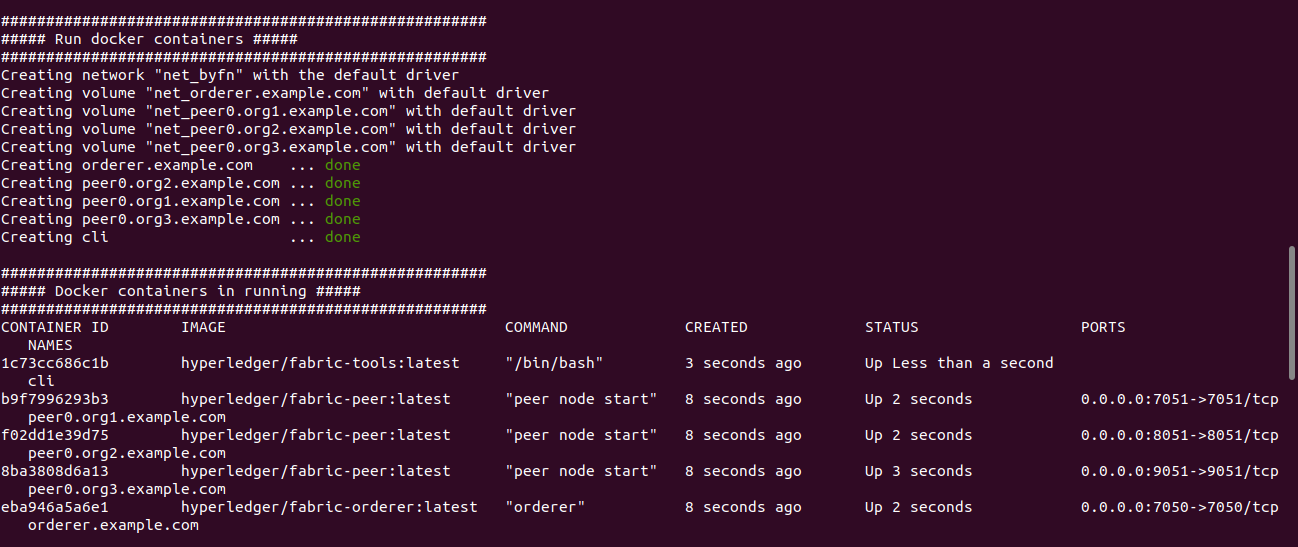
\includegraphics[totalheight=6cm]{img/network/net-1.png}
    \caption{Run of the Docker Containers}
    \label{fig:docker-run}
\end{figure}

\begin{figure}[!ht]
    \centering
    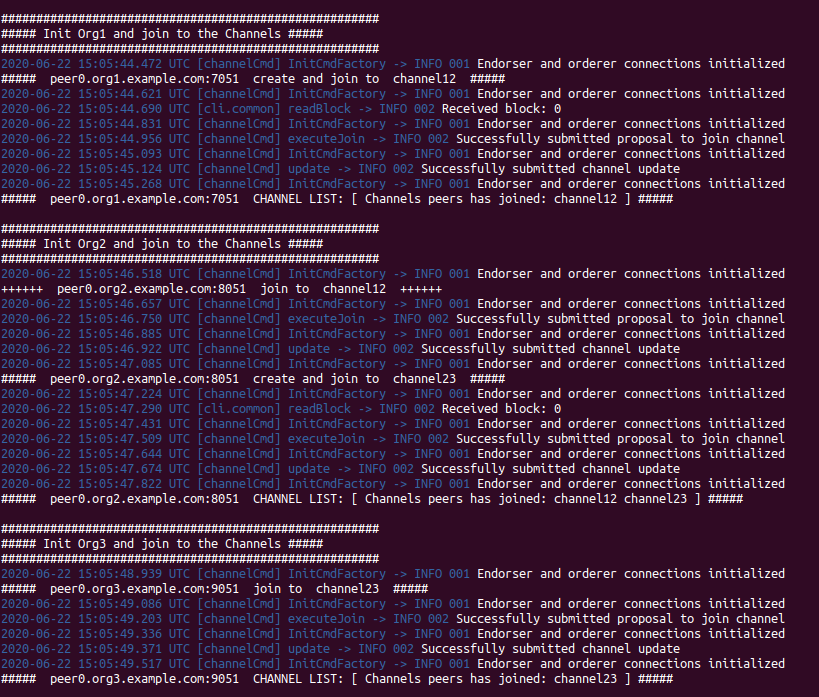
\includegraphics[totalheight=8cm]{img/network/net-2.png}
    \caption{Orgs initializations and channels join}
    \label{fig:init-org}
\end{figure}

\begin{figure}[!ht]
    \centering
    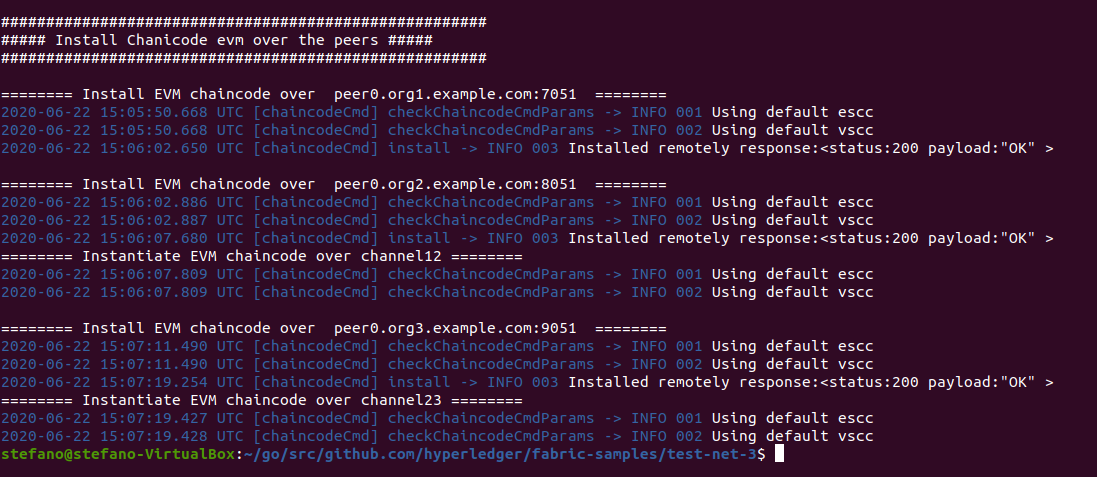
\includegraphics[totalheight=6cm]{img/network/net-3.png}
    \caption{Chaincode Installation}
    \label{fig:install-chaincode}
\end{figure}

\subsubsection{Scripts produced}

For a better understanding of the setting up and running of the entire network i reported below
the two main script. The two files \textbf{\texttt{net\_up.sh}} and \textbf{\texttt{net\_down.sh}}
show in the best way all the steps that allow the network running.

\textbf{\texttt{net\_up.sh}}:

\begin{lstlisting}[language=bash]
    #!/bin/bash

    #Generate crypto material for organizations
    echo "######################################################"
    echo "##### Generate Crypto Material for Organizations #####"
    echo "######################################################"
    ../bin/cryptogen generate --config=./crypto-config.yaml

    # Build channel artifact
    echo "######################################################"
    echo "##### Build Channel Artifact #####"
    echo "######################################################"
    ./channel_artifact.sh


    # Run up docker containers
    echo
    echo "######################################################"
    echo "##### Run docker containers #####"
    echo "######################################################"
    docker-compose up -d

    echo "######################################################"
    echo "##### Docker containers in running #####"
    echo "######################################################"
    docker ps

    # Org1 Initialization and join channels
    echo "######################################################"
    echo "##### Init Org1 and join to the Channels #####"
    echo "######################################################"
    docker exec cli scripts/org1_init.sh

    # Org2 Initialization and join channels
    echo "######################################################"
    echo "##### Init Org2 and join to the Channels #####"
    echo "######################################################"
    docker exec cli scripts/org2_init.sh

    # Org3 Initialization and join channels
    echo "######################################################"
    echo "##### Init Org3 and join to the Channels #####"
    echo "######################################################"
    docker exec cli scripts/org3_init.sh

    # Install and Instantiate evmcc
    echo
    echo "######################################################"
    echo "##### Install Chanicode evm over the peers #####"
    echo "######################################################"
    docker exec cli scripts/install.sh
\end{lstlisting}

\bigskip

\textbf{\texttt{net\_down.sh}}:

\begin{lstlisting}[language=bash]
    #!/bin/bash

    # STOP AND DELETE THE DOCKER CONTAINERS
    docker-compose down -v
    docker rm $(docker ps -aq)
    docker rmi $(docker images dev-* -q)

    # DELETE THE OLD DOCKER VOLUMES
    docker volume prune

    # DELETE OLD DOCKER NETWORKS (OPTIONAL: seems to restart fine without)
    docker-compose -f  down --volumes --remove-orphans
    docker network prune

    # DELETE SCRIPT-CREATED FILES
    rm -rf channel-artifacts/*.block channel-artifacts/*.tx crypto-config

    # Remove creted folder
    rm -rf channel-artifacts

    # VERIFY RESULTS
    docker ps -a
    docker volume ls
    ls -l
\end{lstlisting}

\newpage
\subsection{Ethereum Network - Ropsten}

To run the ERC20 token it's used the testnet Ropsten against the mainnet. 
To set up and upload own ERC20 Token over the ethereum network it's used:

\begin{outline}
    \1 \textbf{My Ether Wallet}: To upload ERC20 contract 
    \1 \textbf{Etherscan.io}: To monitor and analyze transactions over the network
    \1 \textbf{Metamask}: To create user wallets and sign eth transactions
    \1 \textbf{Infura}: To set up a node in order to use it as endpoint and communicate with the Ropsten network,
    it is used as \textit{Provider} in \textit{Web3} library.  
\end{outline}

\section{Fabric and EVM chaincode interaction}

\subsection{Chaincode invocation}

To analyze how evm chaincode allow to run Solidity bytecode inside Hyperledger Fabric network, first
of all we're going to analyze the interaction process and chaincode invocation Process of Hyperledger 
Fabric Blockchain. 

\subsubsection{End to End Interactions} 
Going deeper, the \textbf{Figure \ref{fig:end_to_end}} show the flow of the end to end communication. How all the components are boxed 
inside the Peer component. The Fab3 map the web3 request and forward it to fabric peer. the request 
arrive to the evmcc that invoke Solidity smart contract methods.

\begin{figure}[h!]
    \centering
    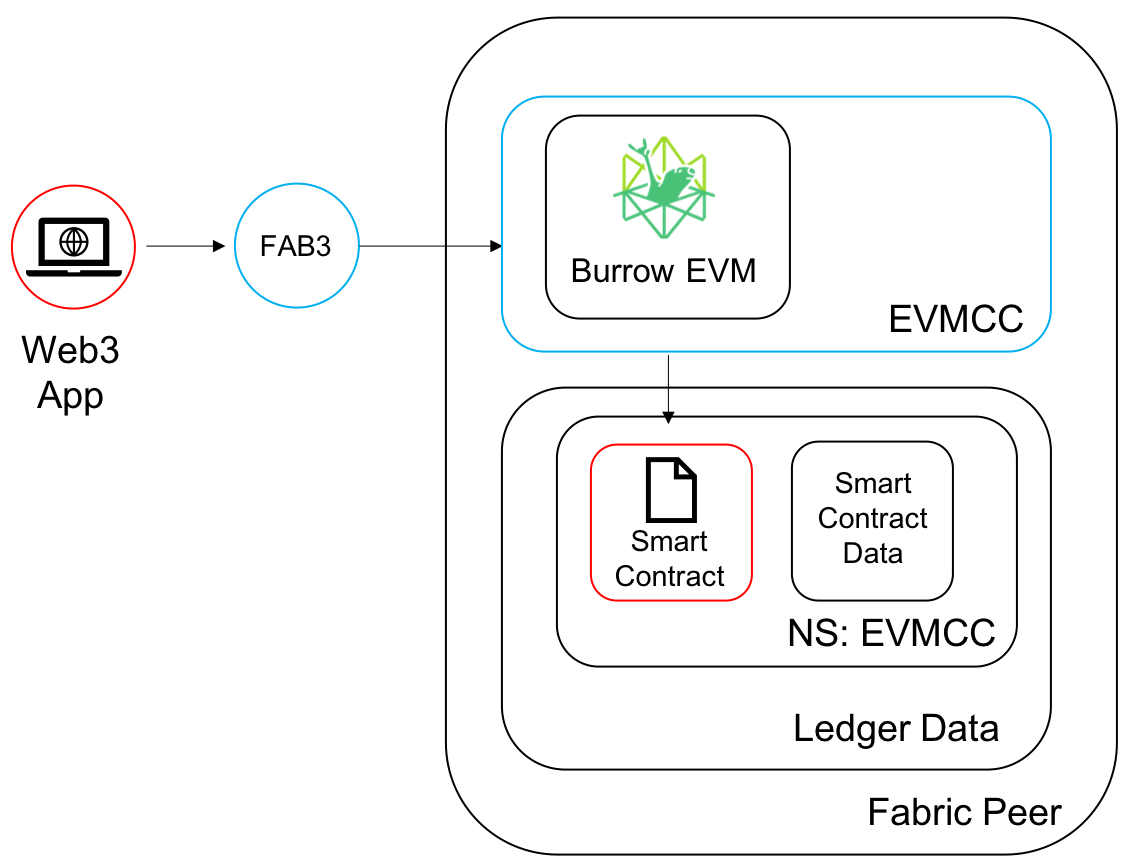
\includegraphics[totalheight=7.5cm]{img/EndToEnd.png}
    \caption{End To End}
    \label{fig:end_to_end}
\end{figure}

\subsubsection{Chaincode Invocations}
The \textbf{Figure \ref{fig:sc_invokation}} below describe the internal workflow of the chaincode invocation, where's involved the 
\textit{Client} the \textit{Peer} and the \textit{Orderer}. All the information are transfer over the 
setted channel and in our study case, the client doesn't interact directly, but using \textit{Fab3 Proxy}
as intermediary.

\begin{figure}[h!]
    \centering
    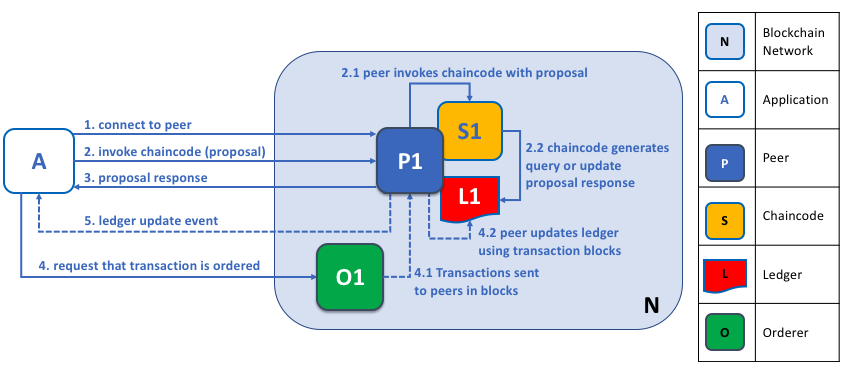
\includegraphics[totalheight=6cm]{img/sc_invokation.png}
    \caption{Smart Contract Invocation Process}
    \label{fig:sc_invokation}
\end{figure}

\newpage
\subsection{Fab3 Proxy}

The Fab3 Proxy is a main component of the entire architecture. It works as a bridge between the Ethereum
world and the Hyperledger Fabric one. Each instance of Fab3 going to map 1 fabric user and going to 
generate a semi random eth address starting from the public key of own x.509 certificate related to
Fabric identity. 
The Following environment variable going to set the mandatory data to run a Fab3 proxy instance:

\begin{outline}
    \1 \textbf{CONFIG}: It's the path to a compatible Fabric SDK Go config file, used to communicate and map the requests and forard it to fabric network.
    \1 \textbf{USER}: User identity being used for the proxy. Matches the users names in the crypto-config directory specified in the config.
    \1 \textbf{ORG}: Organization of the specified user.
    \1 \textbf{CHANNEL}: Channel to be used fo the transactions.
    \1 \textbf{CCID}: ID of the EVM chaincode deployed in your fabric network.
    \1 \textbf{PORT}: Port the proxy will listen on. If not provided default is 5000
\end{outline}

\begin{lstlisting}
# Environment variables required for setting up Fab3
export FAB3_CONFIG=${GOPATH}/src/github.com/hyperledger/fabric-chaincode-evm/examples/network-sdk-config.yaml 
export FAB3_USER=User1 
export FAB3_ORG=Org1
export FAB3_CHANNEL=channel12 
export FAB3_CCID=evmcc
export FAB3_PORT=5000
\end{lstlisting}

Once the fab3 is set up and the instance is in running we could perform chaincode invocation using 
our Dapp. The \textbf{Figure \ref{fig:fab3_flow}} shows the flow of the invocation process at upper level,
It shows the main components that are involved in that process, 

\begin{outline}[enumerate]
    \1 \textbf{Dapp} call method that perform smart contract invocation.
    \1 \textbf{Fab3} map the request and forward it to Fabric network.
    \1 \textbf{Fabric network} process the request and issue a response.
\end{outline}

\begin{figure}[h!]
    \centering
    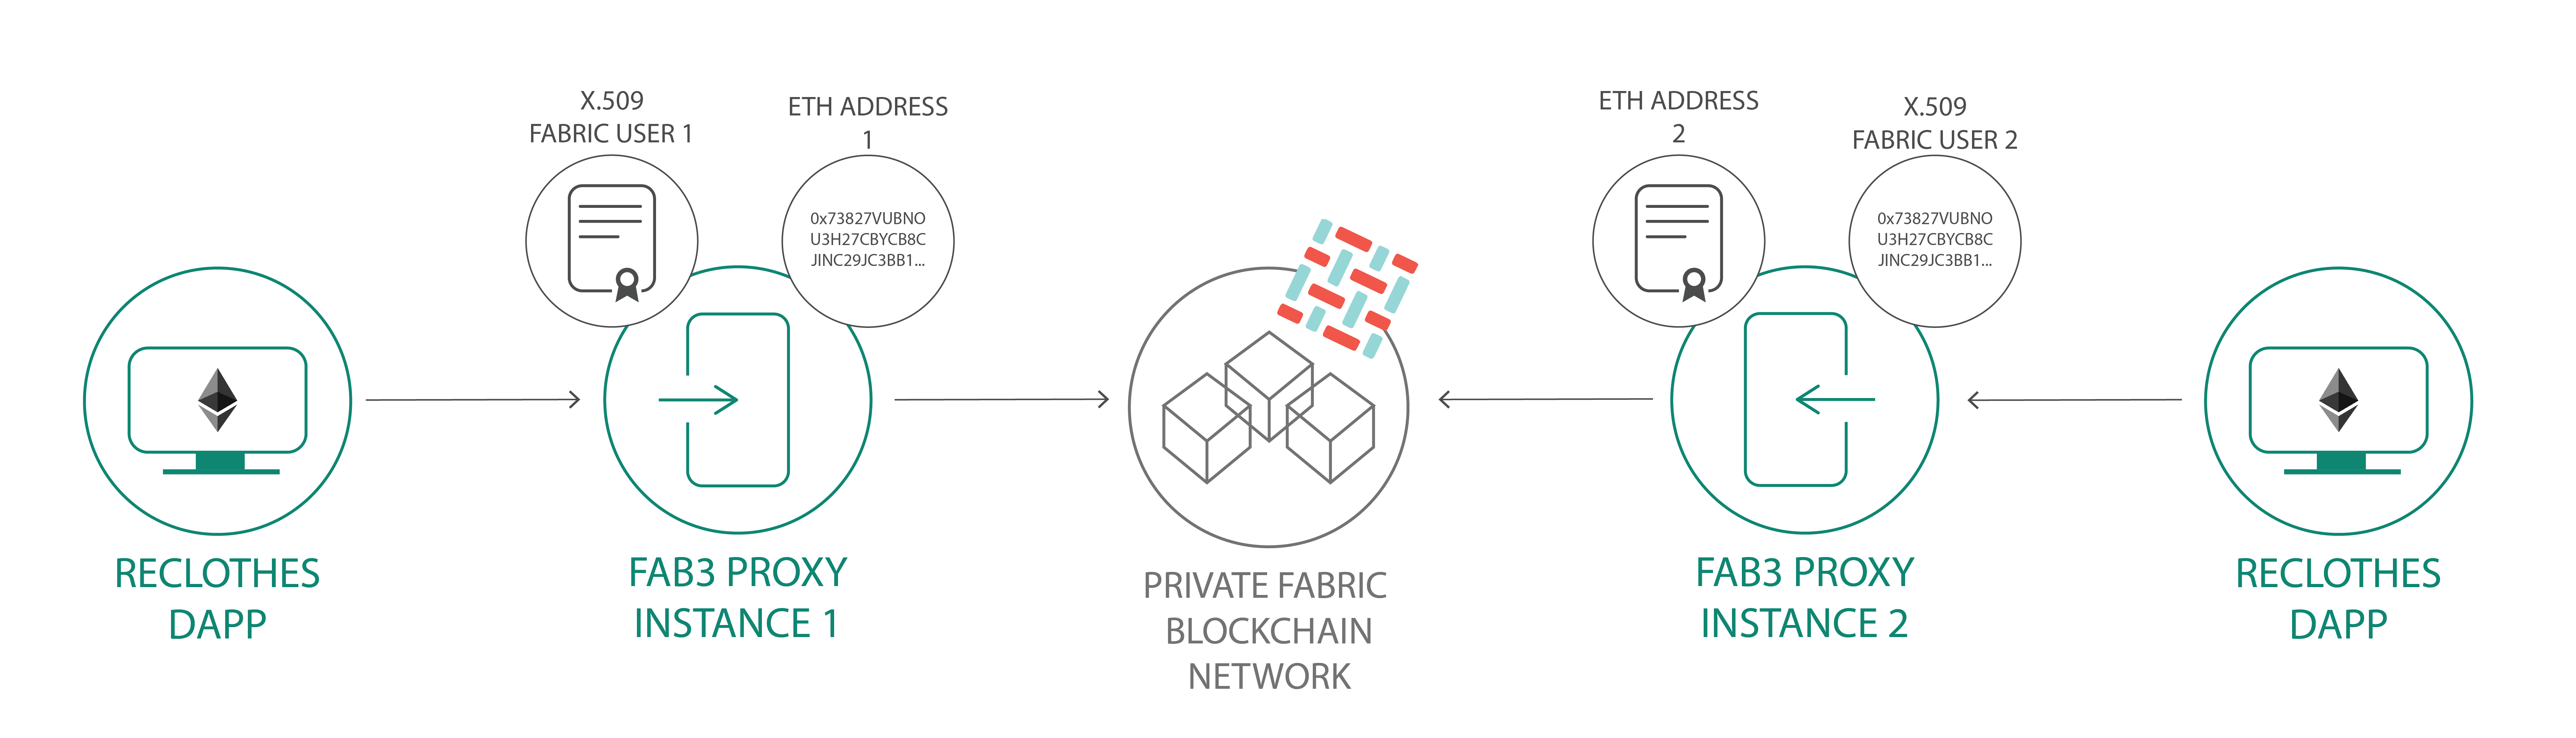
\includegraphics[totalheight=5cm]{img/fab3_flow.png}
    \caption{Fab3 Proxy Flow}
    \label{fig:fab3_flow}
\end{figure}

The \textbf{Figure \ref{fig:fab3_invokation}} show the internal components that take part to the invocation
process. Fab3 agreed the request using \textit{Ethereum JSON RPC API} map it and forward to the fabric
network using \textit{GO SDK}. Once the request arrive to \textit{EVMCC} it invoke smart contract bytecode
and than follow the standard process explained in Figure \ref{fig:sc_invokation}.

\begin{figure}[h!]
    \centering
    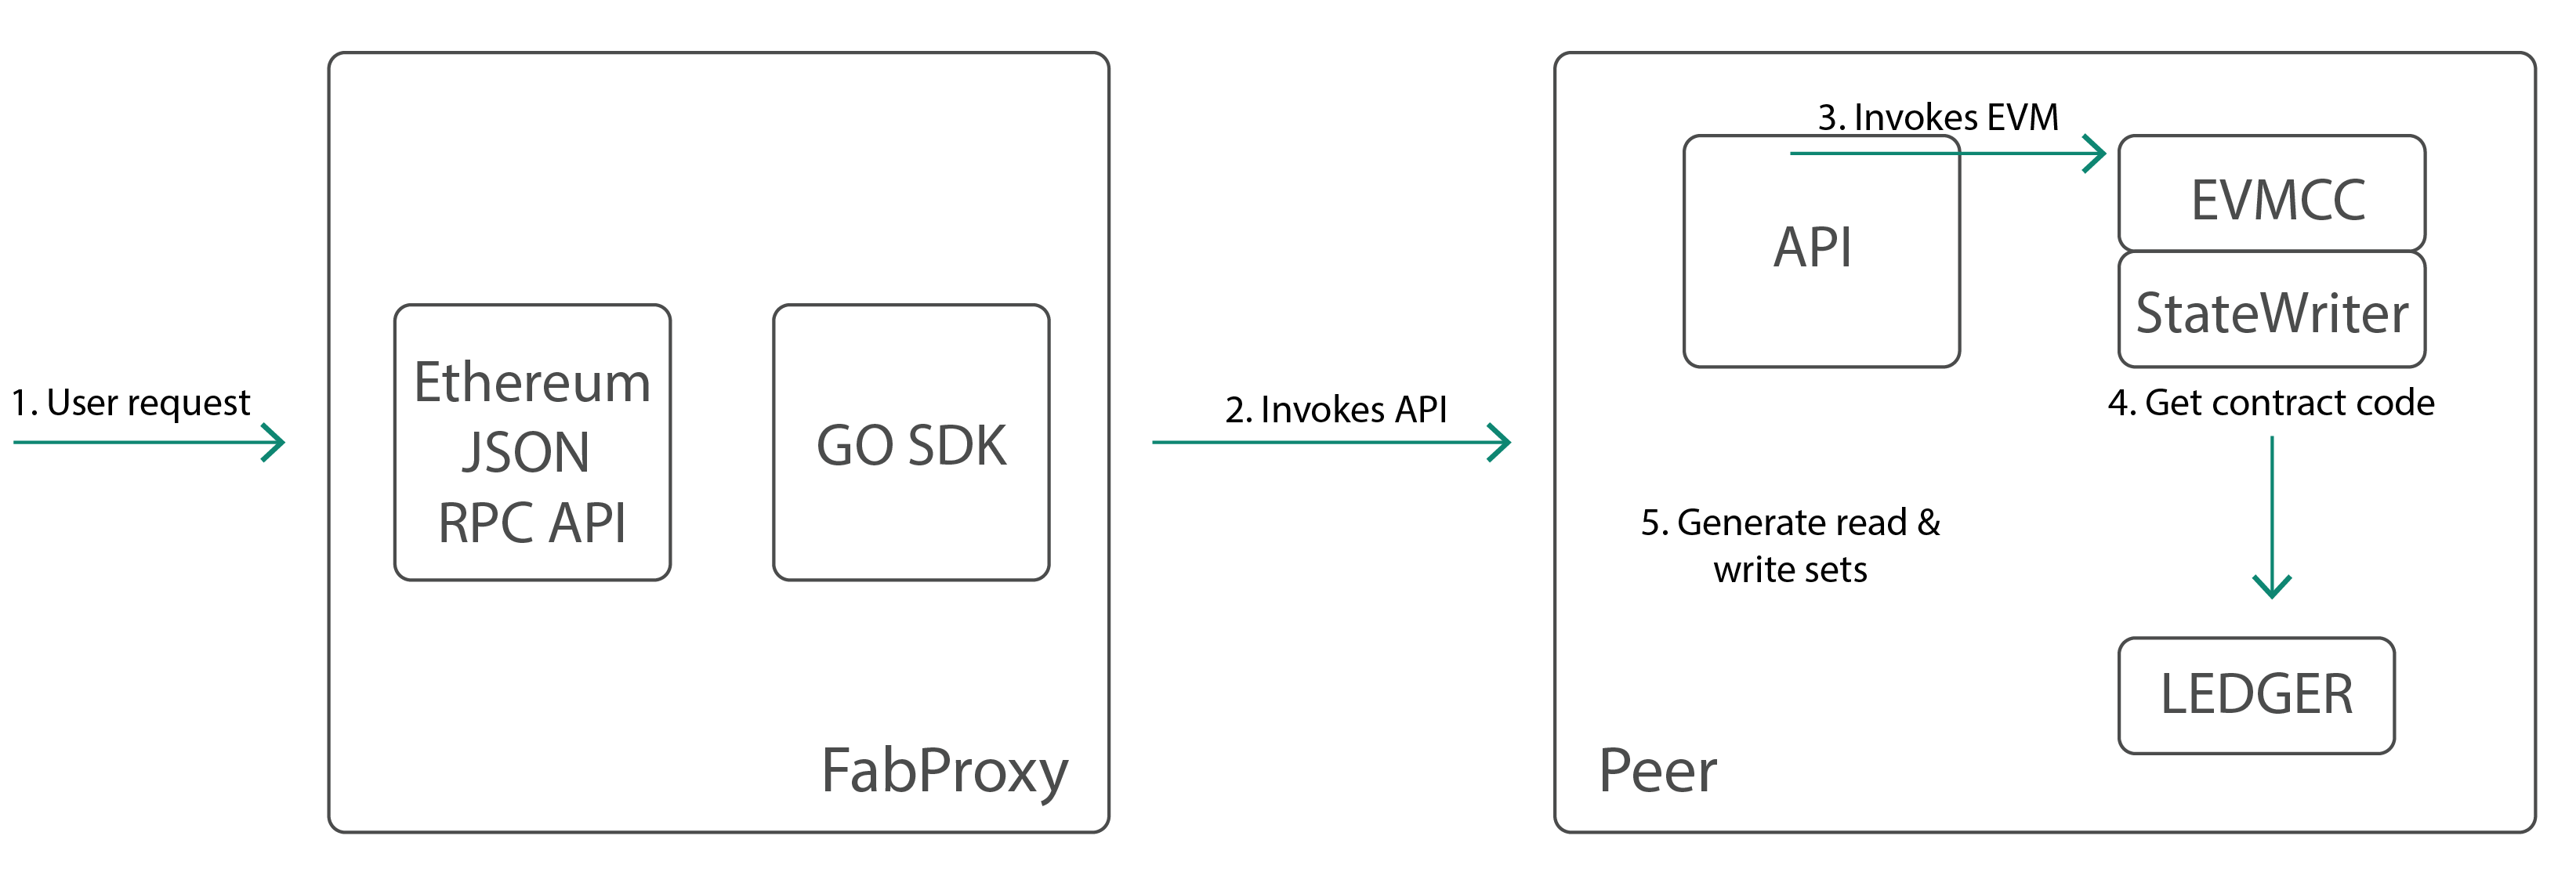
\includegraphics[totalheight=5cm]{img/fab3_invokation.png}
    \caption{Fab3 Invocation Process}
    \label{fig:fab3_invokation}
\end{figure}


% DAPP
\newpage
\section{Dapp}

\subsection{Technologies used}

The client application is a web app, composed by a front-end part and a mid level with API that allow
the comunication with smart contracts of both Blockchains. The technologies used are the following one:

\begin{outline}
    \1 \textbf{Expressjs}: It's a node.js framework that allow to develop api for own application
    \1 \textbf{Bootstrap}: To build a user friendly front-end in order to interact in the best way
    \1 \textbf{Web3}: Ethereum Javascript API, It's is a collection of libraries that allow you to interact with a local or remote ethereum node 
    \2 \textbf{web3 0.20.2}: used for dapp developments, fabric side, It's a stable version and it's the version
    used in \texttt{fabric-chaincode-evm} development
    \2 \textbf{web3 1.0.0}: used for ethereum transactions, It's a version with more functionalities but less stable.
\end{outline}

Starting from the Homepage the User is allowed to register itself as \textbf{User}, \textbf{Reclothes Admin}
or \textbf{Producer}.

\subsection{Core part of the web-app}

The technical files and flow that dapp follow to run up it's the following one.

\begin{outline}[enumerate]
    \1 \textbf{Contract Address Generation}:
    \2 This step is in charge to run a script that deploy the contract adresses to be reffered during the 
    app running.
    \3 \textbf{UserContract.js}: running the script using \texttt{node .js file}, it return the address of the deployed contract.
    The \textbf{Figure \ref{fig:deploy-user-contract}} show the related output and the Contract Address
    printed. 
    \3 \textbf{ProducerContract.js}: running the script using \texttt{node .js file}, it return the address of the deployed contract.
    The deployed process and output is similar to Figure \ref{fig:deploy-user-contract}.
    \1  \textbf{dapp.js}: there's the core file that handle the contracts invokations, set up the contract address
    referance, and connect to a specific Fab3 instance.
    \1 \textbf{app.js}: It set up the API called by the web-app, map the request and forward to \texttt{dapp.js}.
\end{outline}

\begin{figure}[h!]
    \centering
    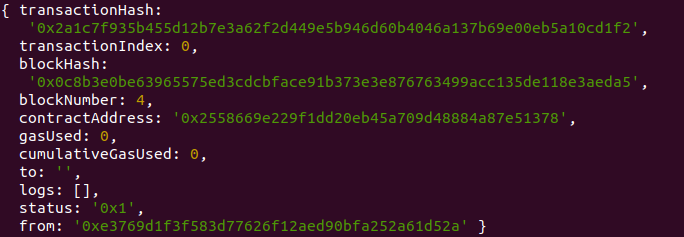
\includegraphics[totalheight=4cm]{img/app-running/deployUserContract.png}
    \caption{Deploy User Contract}
    \label{fig:deploy-user-contract}
\end{figure}

Once is all set up we could run the web-app with the command \texttt{npm start}, there's an initializzation
phase and that the app is ready to use and in running of over the specified PORT. The \textbf{Figure \ref{fig:app-running}}
shows the output. 

\begin{figure}[h!]
    \centering
    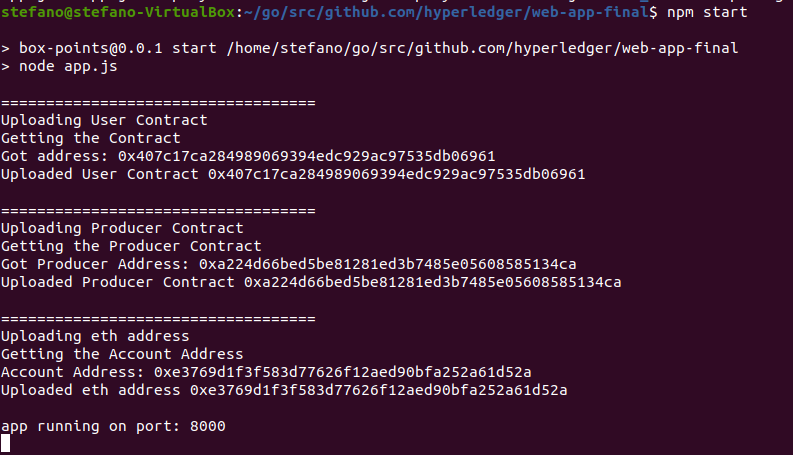
\includegraphics[totalheight=6cm]{img/app-running/app-running.png}
    \caption{App Running}
    \label{fig:app-running}
\end{figure}

\newpage
\subsection{Views}

\subsubsection{Homepage}

The homepage allow user to view the feature of each User type and to access to the registration page.

\begin{figure}[h!]
    \centering
    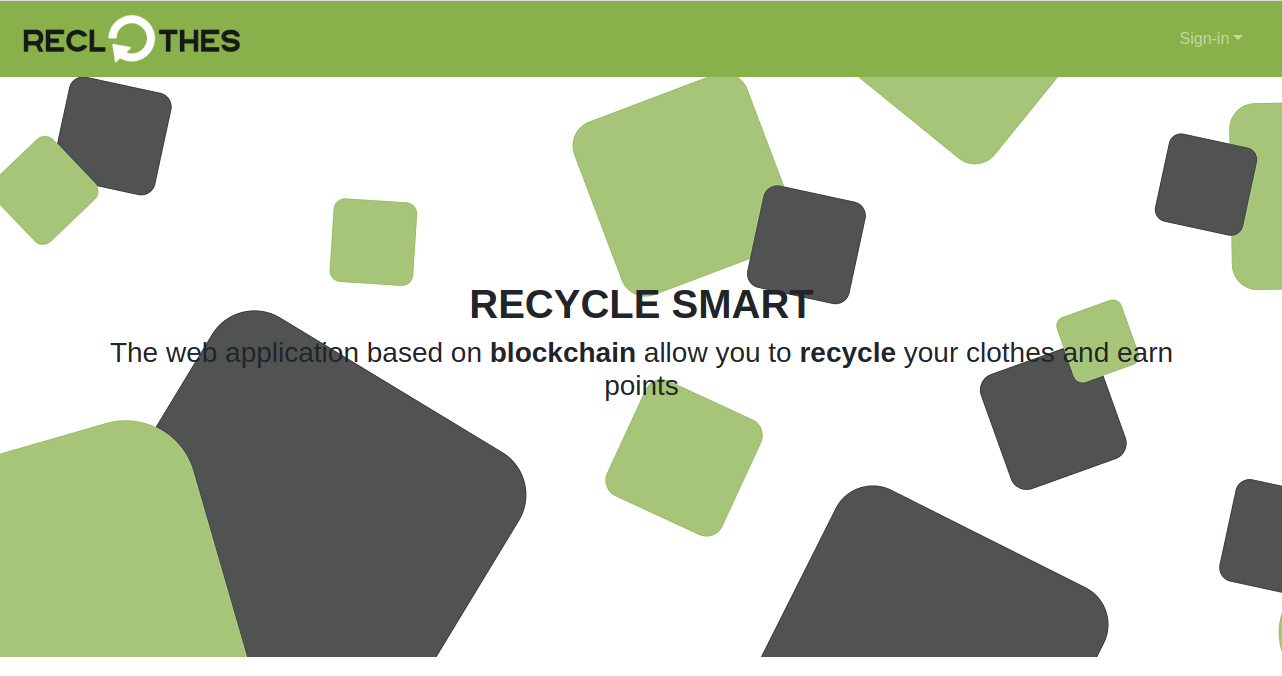
\includegraphics[totalheight=7.5cm]{img/dapp/home1.png}
    \caption{Home}
    \label{fig:home}
\end{figure}

\begin{figure}[h!]
    \centering
    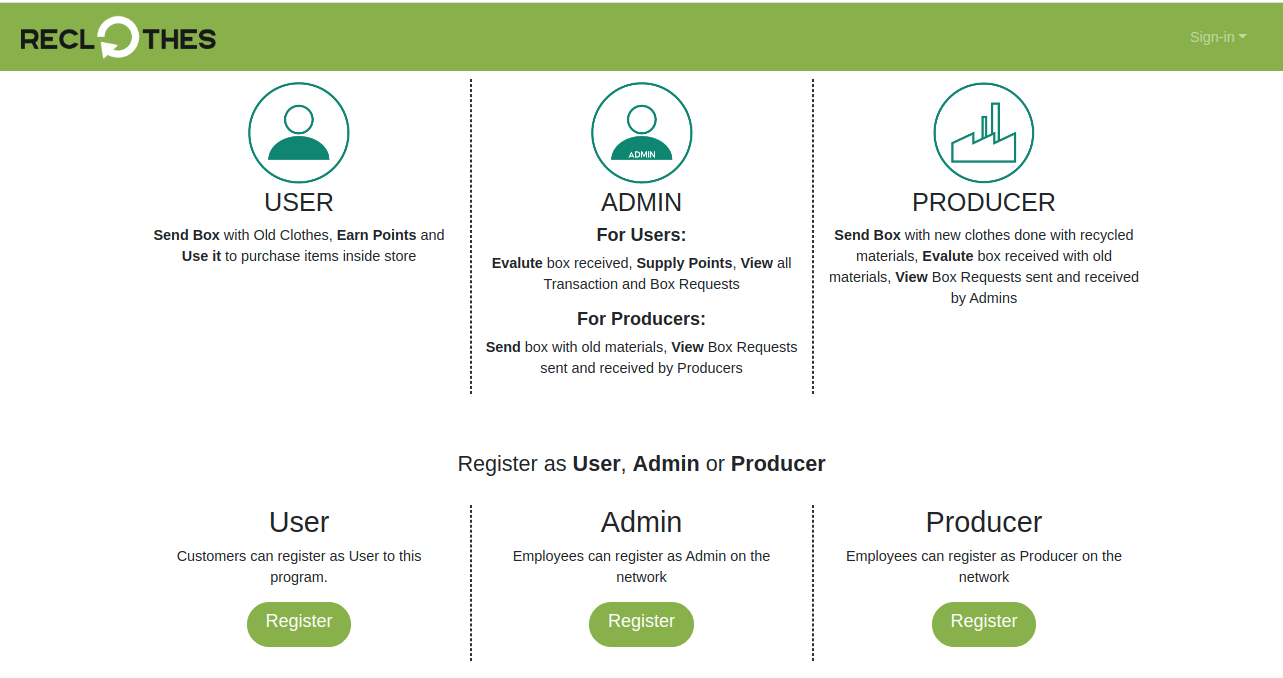
\includegraphics[totalheight=7.5cm]{img/dapp/home2.png}
    \caption{Registration Phase}
    \label{fig:registration}
\end{figure}

\newpage
\subsubsection{User Page}

The User page allow to view an overview infos once the user is logged in. 

\begin{enumerate}[-]
    \item \textbf{Address}: It's the public eth address setup during registration phase. 
    \item \textbf{Points Balance}: It's the Fabric points balance earned by the user sending the boxes.
    \item \textbf{ERC20 Balance}: It's the eth balance of the public token running over eth network.
\end{enumerate}

The \textbf{Figure \ref{fig:send_box}} show how to compile the form in order to send box with old clothes. It's a simulation
of the real process to sending box, that in the real case could be implemented thow a QRCode or RFID
placed over the boxes.

The \textbf{Figure \ref{fig:purchase_clothes}} show how should be the store, purchase items over the platform start the transaction 
process. 

There's other section about infos that user is allowed to see. \textbf{Transactions} performed over
the fabric network and \textbf{Box Requests} that's all the history about the box sent and received
with all the related informations. 

\begin{figure}[h!]
    \centering
    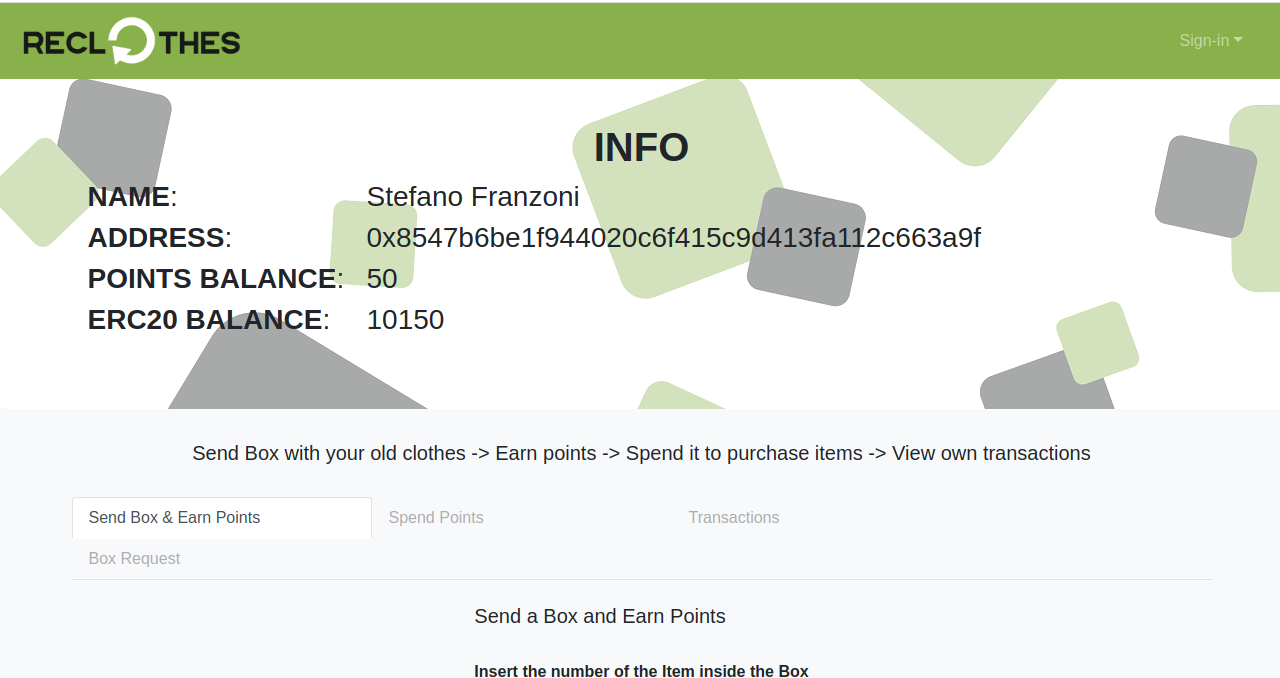
\includegraphics[totalheight=7.5cm]{img/dapp/user-info.png}
    \caption{User Info}
    \label{fig:user_info}
\end{figure}

\begin{figure}[h!]
    \centering
    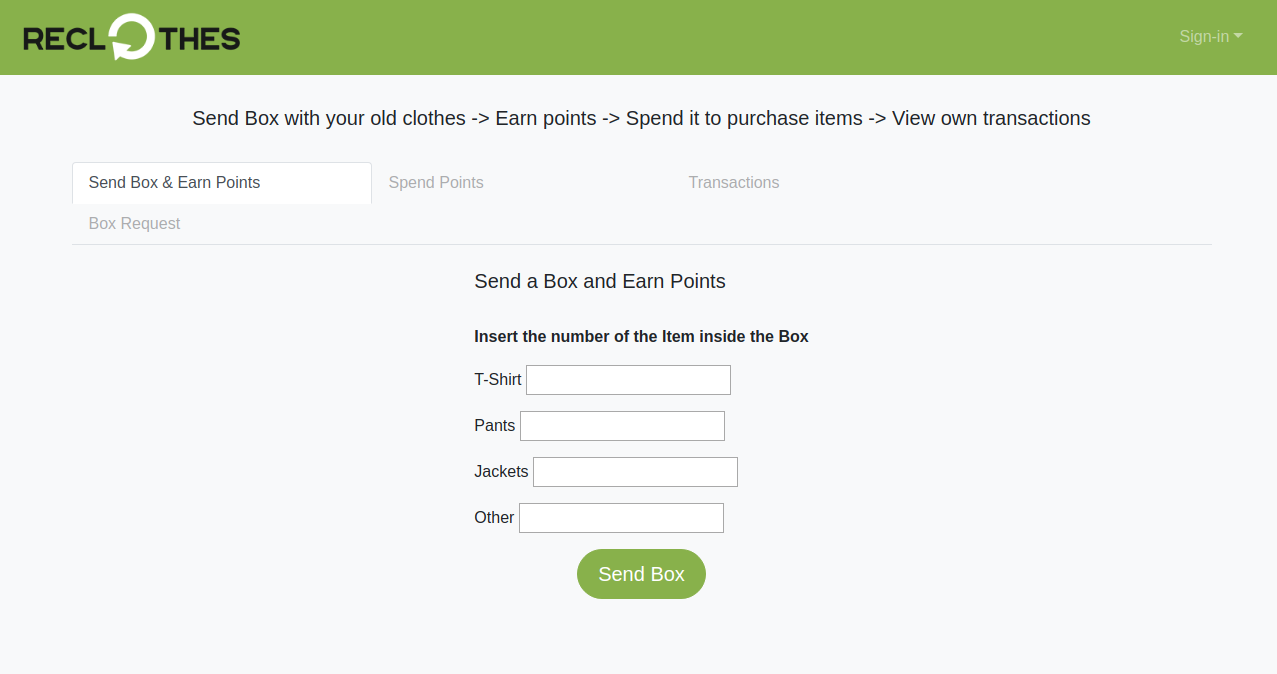
\includegraphics[totalheight=7.5cm]{img/dapp/user-send.png}
    \caption{Send Box}
    \label{fig:send_box}
\end{figure}

\begin{figure}[h!]
    \centering
    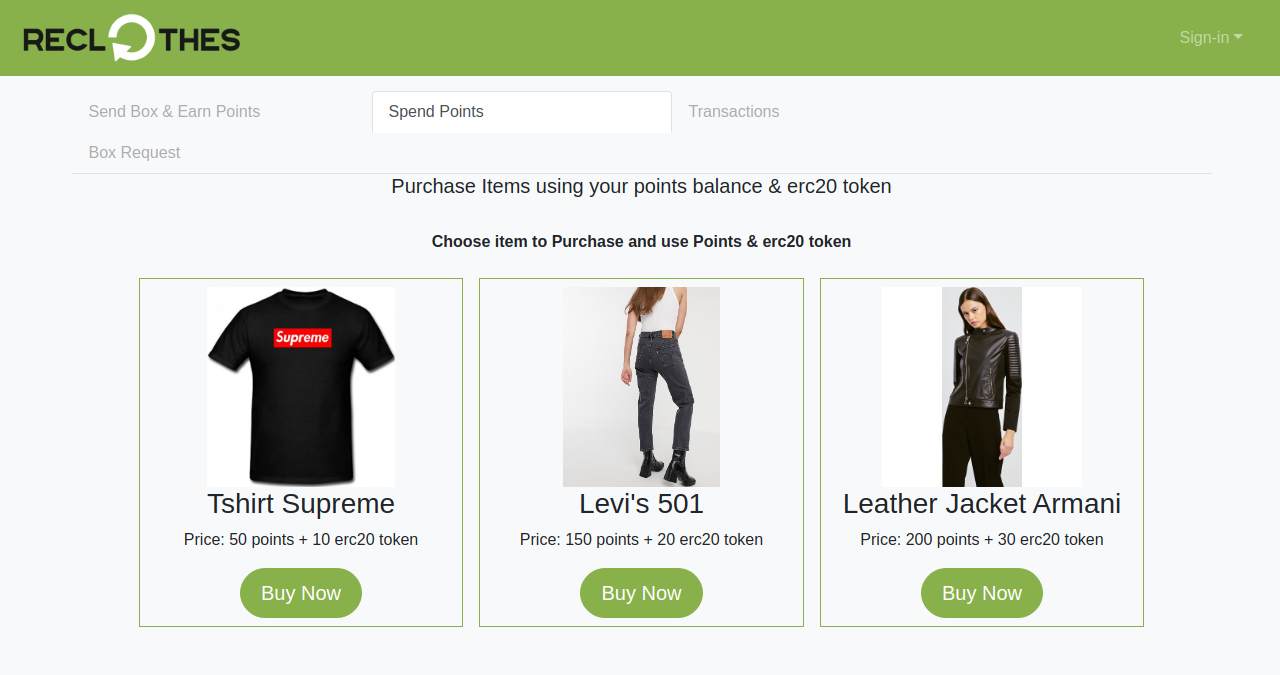
\includegraphics[totalheight=7.5cm]{img/dapp/user-buy.png}
    \caption{Purchase Clothes}
    \label{fig:purchase_clothes}
\end{figure}

\newpage
\subsubsection{Reclothes Admin Page}

In the previous sections we talk about a logical split about Admin for User and Admin for Producers.
In the following views we divide the feature releated to the User type to be handled and there's a 
streight distinctions about Users and Producers.

\paragraph{Admin For Users}

This section show the view of the Admins that handle User side.

\begin{figure}[h!]
    \centering
    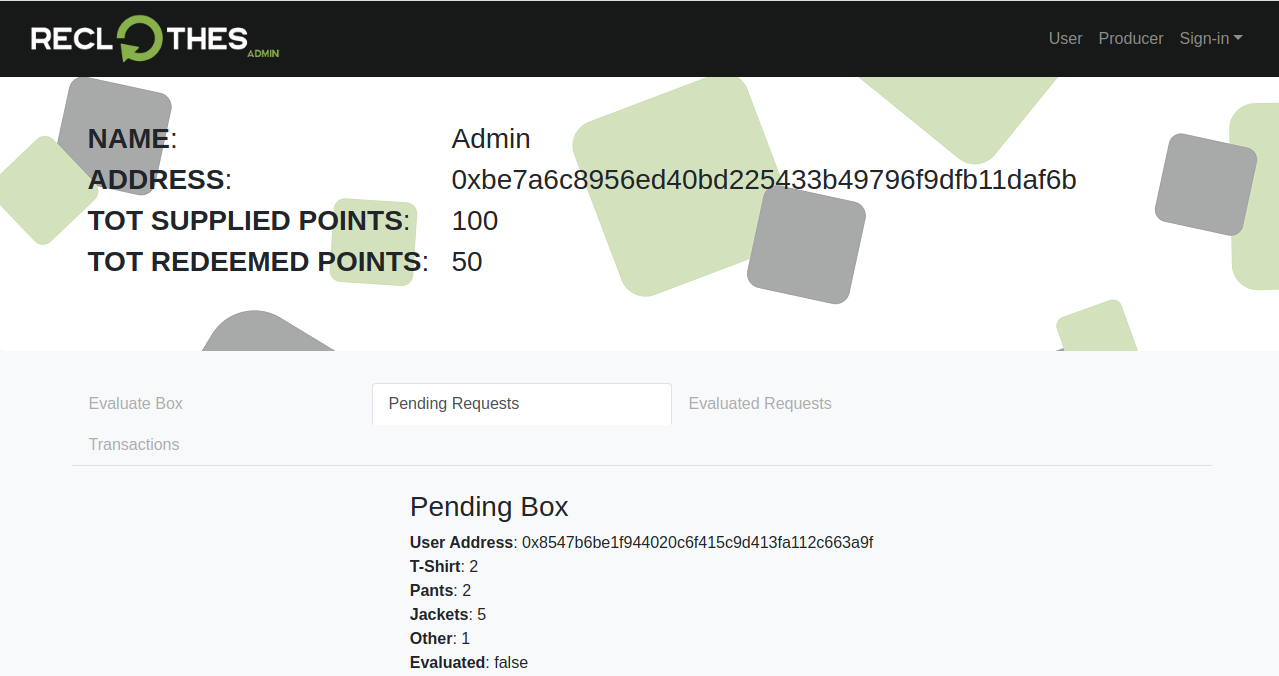
\includegraphics[totalheight=7.5cm]{img/dapp/admin-info.png}
    \caption{Admin Info}
    \label{fig:admin_info}
\end{figure}

\begin{figure}[h!]
    \centering
    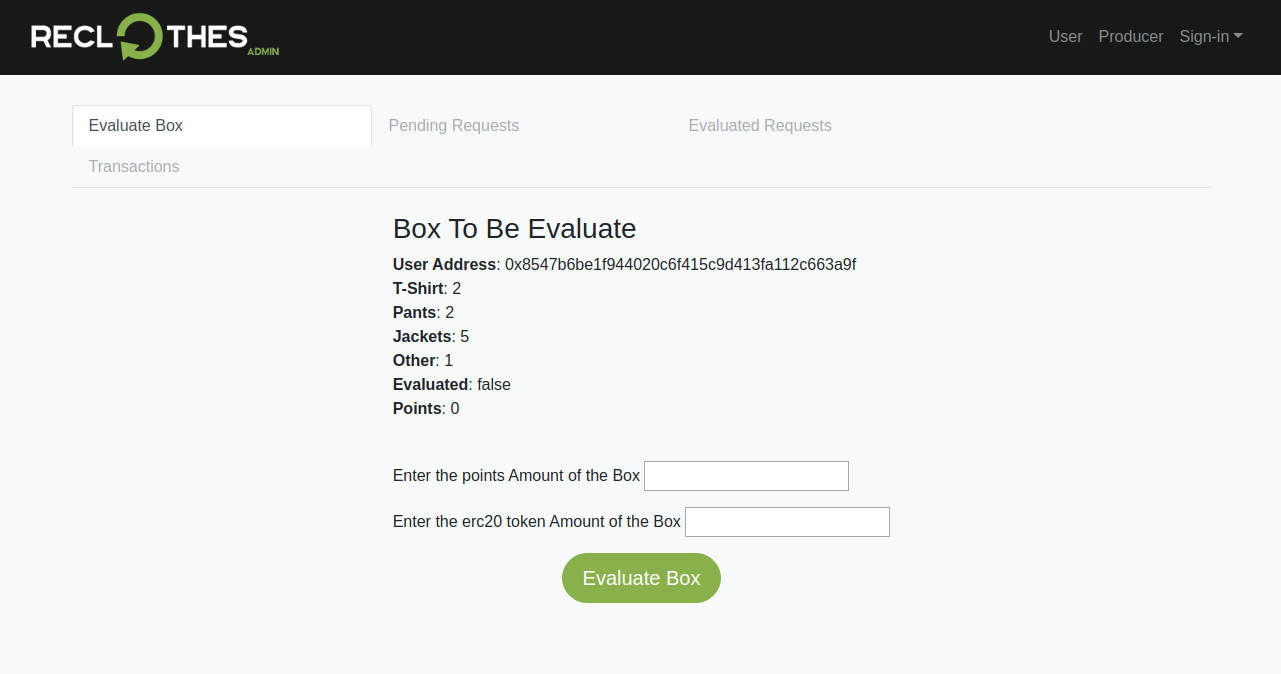
\includegraphics[totalheight=7.5cm]{img/dapp/admin-evaluate.png}
    \caption{Evaluate Box}
    \label{fig:evaluate_box}
\end{figure}

\begin{figure}[h!]
    \centering
    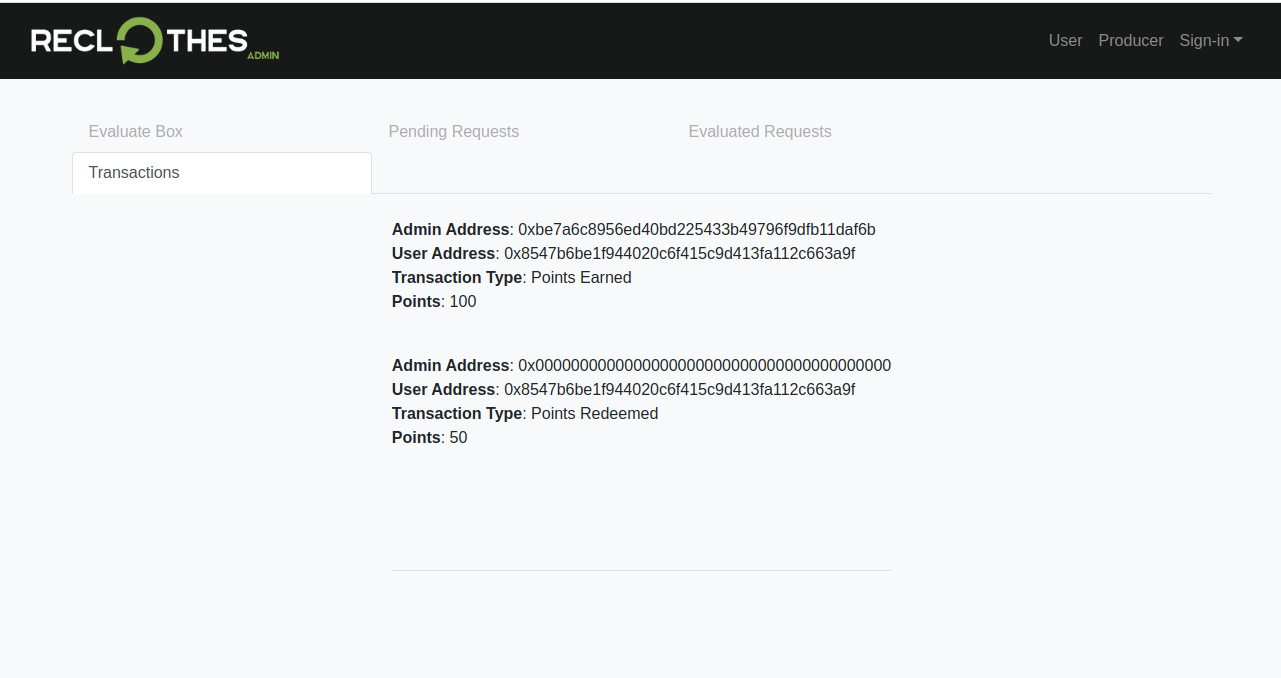
\includegraphics[totalheight=7.5cm]{img/dapp/admin-tx.png}
    \caption{Transactions}
    \label{fig:admin-tx}
\end{figure}

\paragraph{Admin For Producers}

This section show the view of the Admins that handle Producer side. The Figure \ref{fig:adminp-info} 
show all the Admin for Producers informations. 

\begin{figure}[h!]
    \centering
    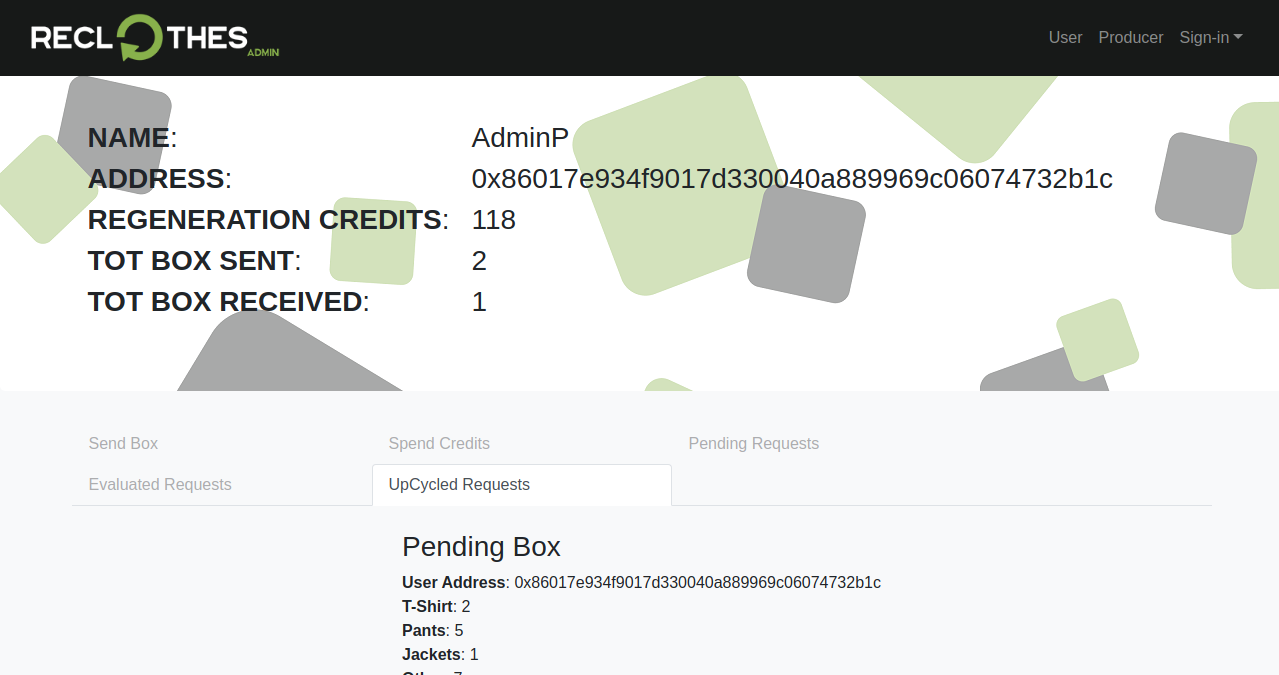
\includegraphics[totalheight=7.5cm]{img/dapp/adminp-info.png}
    \caption{Admin for Producers Info}
    \label{fig:adminp-info}
\end{figure}

\begin{figure}[h!]
    \centering
    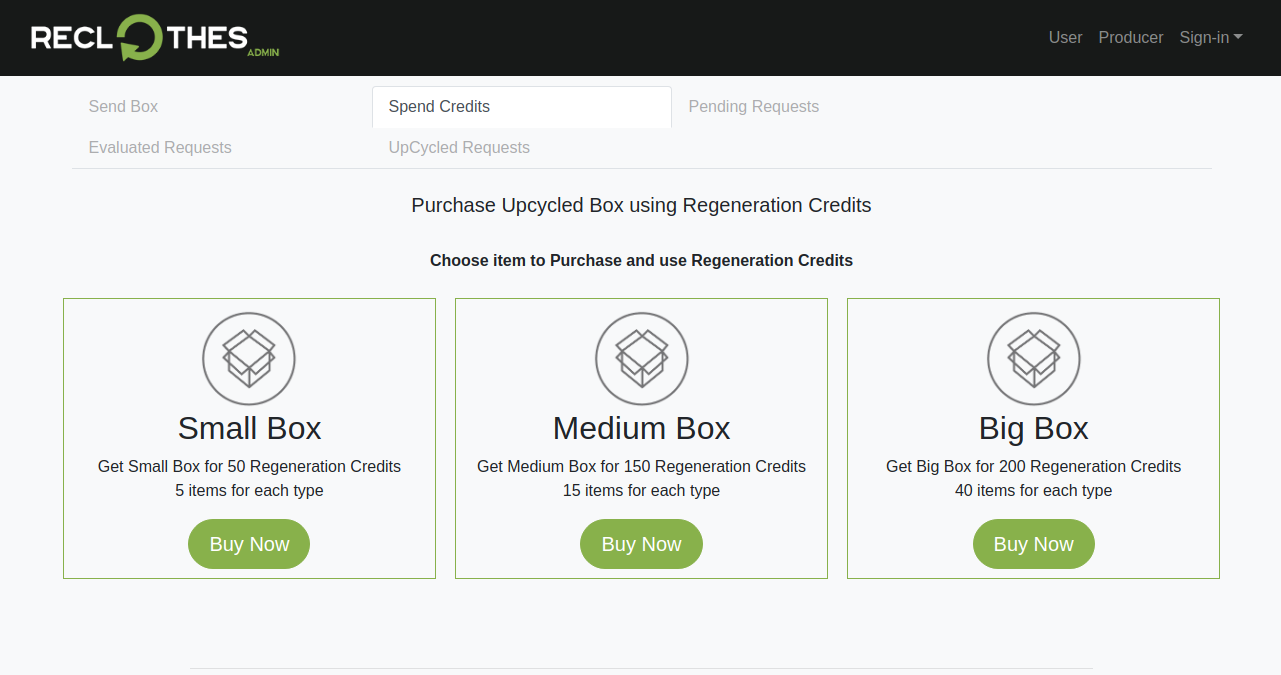
\includegraphics[totalheight=7.5cm]{img/dapp/adminp-buy.png}
    \caption{Admin Spend Regeneration Credits}
    \label{fig:adminp-buy}
\end{figure}

\newpage
\subsubsection{Producer}

This section show the view of the Producer side. The evaluation process of the old materials
received buy Reclothes it's the same of the previous one.

\begin{figure}[h!]
    \centering
    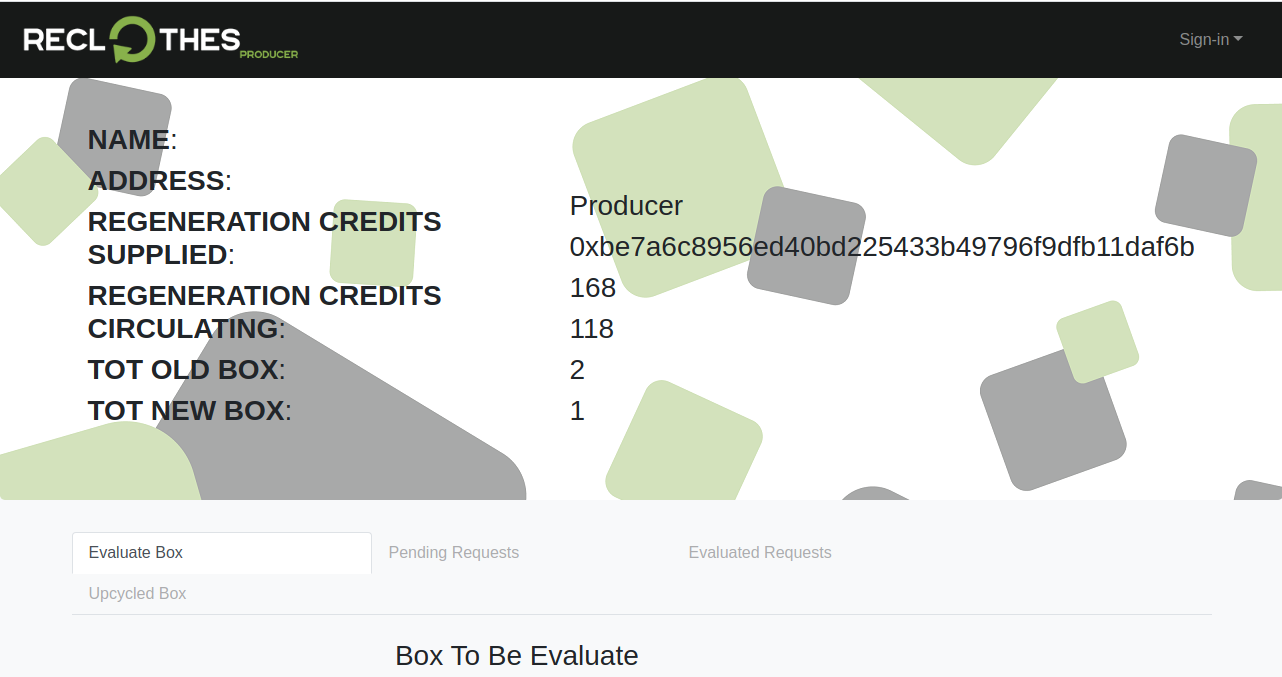
\includegraphics[totalheight=7.5cm]{img/dapp/producer-info.png}
    \caption{Producers Info}
    \label{fig:producer-info}
\end{figure}
